\section{Neural networks}
%Background biologico
\subsection{Background biologico}
Il nostro cervello è in grado di analizzare in modo sofisticato l'ambiente circostante per agire in modo efficace, come il riconoscimento e la reazione ad un pericolo. Lo studio di questi processi coinvolge biologia, medicina e psicologia. Ciò ha portato alla \uline{creazione di modelli che simulano l'attività cerebrale, utilizzati dall'informatica per offrire strumenti di predizione, ottimizzazione e problem-solving in vari campi applicativi}. Il successo di questi modelli dipende dalla capacità di elaborare grandi quantità di dati in parallelo.

Il sistema nervoso degli animali è composto dal cervello (che nelle forme di vita "inferiori" viene spesso chiamato solo "sistema nervoso centrale"), dai diversi sistemi sensoriali che raccolgono informazioni dalle diverse parti del corpo e dal sistema motorio che controlla i movimenti. La maggior parte dell'elaborazione delle informazioni avviene nel cervello/sistema nervoso centrale. Il cervello è composto da miliardi di cellule dette \textit{neuroni}.
Un neurone è una cellula che raccoglie e trasmette attività elettrica ed è costituito da:
\begin{itemize}
    \item \textit{soma}, corpo cellulare del neurone che contiene il nucleo
    \item \textit{dendriti}, sono filamenti raggiunti dalle terminazioni di altri neuroni e che gli permettono di raccogliere informazioni grazie a processi biochimici originati dai così detti neuro-trasmettitori
    \item \textit{assone}, un lungo filamento (da alcuni millimetri a un metro) che si estende dal corpo principale della cellula nervosa e trasmette segnali elettrici che attivano altri neuroni attraverso il rilascio di neuro-trasmettitori. E' il percorso fisso lungo il quale i neuroni comunicano tra di loro. Alla sua estremità, l'assone si ramifica e possiede delle estremità chiamate bottoni terminali. Ogni pulsante terminale tocca quasi una dendrite o il corpo cellulare di un altro neurone. (sinapsi)
\end{itemize}
Secondo stime comuni, ci sono circa $100$ miliardi ($10^{11}$) neuroni nel cervello umano, di cui una parte abbastanza grande è attiva in parallelo. I neuroni elaborano le informazioni interagendo tra di loro.

\paragraph{Sinapsi} 
Un luogo in cui un assone e una dendrite si toccano quasi. C'è un piccolo spazio tra $10$ e $50 nm$ di larghezza, una miliardesima di metro ($10^{-9}$mt).

E' una struttura specializzata che permette la comunicazione tra neuroni. Consente il trasferimento da un neurone all'altro o verso una cellula effettore (come un muscolo o una ghiandola). Il trasferimento dell'informazione avviene attraverso segnali chimici chiamati neuro-trasmettitori, che vengono rilasciati dalle terminazioni nervose del neurone pre-sinaptico e si legano ai recettori della membrana del neurone post-sinaptico, generando una risposta elettrica o chimica sul neurone destinatario.

\paragraph{Comunicazione tra neuroni}
La forma più comune di comunicazione tra neuroni è che un bottone terminale dell'assone rilascia determinate sostanze chimiche, chiamate neuro-trasmettitori, che agiscono sulla membrana della dendrite ricevente e ne modificano la polarizzazione\footnote{La polarizzazione si riferisce al livello di carica elettrica presente sulla membrana cellulare del neurone. La membrana cellulare è polarizzata quando vi è una differenza di potenziale elettrico tra l'interno e l'esterno della cellula} (il suo potenziale elettrico). Quando questo impulso nervoso raggiunge la fine dell'assone, provoca il rilascio di neuro-trasmettitori nei bottoni terminali, trasmettendo così il segnale alla cellula successiva, dove il processo si ripete.

\begin{figure}[h]
    \centering
    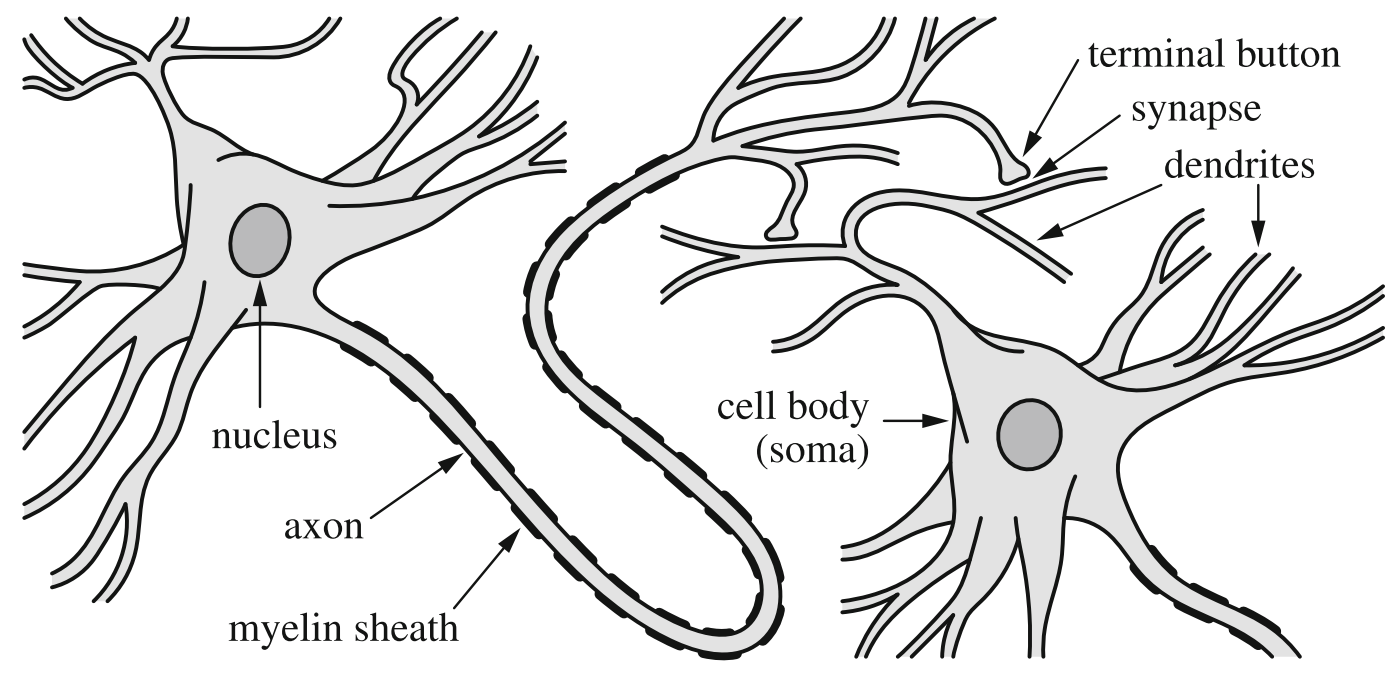
\includegraphics[scale=0.4]{images/neuron.png}
    \caption{Struttura prototipica dei neuroni biologici}
\end{figure}

%Threshold Logic Unit
\subsection{Threshold Logic Unit}
La descrizione delle reti neurali biologiche rende naturale modellare i neuroni come unità logiche a soglia: se un neurone riceve un'input eccitante sufficiente che non viene compensato da un'input inibitorio altrettanto forte, diventa attivo e invia un segnale ad altri neuroni\footnote{Nel contesto della descrizione delle reti neurali biologiche, gli input eccitanti e inibitori rappresentano gli impulsi provenienti da altri neuroni che influenzano l'attività e il comportamento di un neurone specifico. La somma di questi impulsi eccitatori e inibitori determina se il neurone diventerà attivo e invierà un segnale agli altri neuroni.}. Un tale modello è stato già esaminato molto dettagliatamente da McCulloch e Pitts (1943). Di conseguenza, le Threshold Logic Unit sono anche conosciute come \textit{neuroni di McCulloch-Pitts} o \textit{perceptron}.

Per creare una rete neurale artificiale, è necessario trovare \uline{un analogo artificiale del neurone biologico}. Questo ruolo è svolto dalle Threshold Logic Unit, o \textit{TLU}. Una TLU è composta da $n$ variabili di input, indicate con $x1, x2, ..., xn$, e un output $y$. Ad ogni variabile di input è associato un peso, indicato con $w_i$, che rappresenta la sua importanza ai fini del calcolo dell'output della TLU. Inoltre, viene assegnato un threshold $\theta$, che rappresenta la soglia minima di attivazione necessaria per produrre un output positivo.

L'output della TLU viene calcolato mediante una funzione che somma i prodotti tra i pesi delle variabili di input e i loro valori, e confronta il risultato con il threshold $\theta$. Se la somma dei prodotti supera la soglia, l'output della TLU sarà positivo, altrimenti sarà negativo.
$$
y=\begin{cases}
    1 & \text{se } \sum w_ix_i \geq \theta \\
    0 & \text{altrimenti} 
   \end{cases}
$$

\paragraph{AND logico}
Con una TLU, possiamo simulare alcune funzioni booleane, come ad esempio l'AND logico tra due input $x1$ e $x2$. Ciò si ottiene assegnando pesi e threshold in modo da soddisfare un sistema di disequazioni, che definisce una regione nello spazio degli input in cui l'output sarà $1$, e una regione dove sarà $0$

\subsubsection{Interpretazione geometrica}
La formula per calcolare l'output di una TLU è simile all'equazione di un \textit{iperpiano}, che rappresenta un piano in uno spazio di $n$ dimensioni. Un'unità logica a soglia calcola la funzione
$$\sum w_ix_i + \theta = 0 \mathit{\;\;oppure\;\;} \sum w_ix_i - \theta = 0$$

Spesso gli input vengono combinati in un vettore di input $x = (x1, \dots, xn)$ e i pesi in un vettore di peso $w = (w1, \dots, wn)$. Con l'aiuto del prodotto scalare, la condizione testata da una TLU può essere scritta anche come $wx \geq \theta$. E' un interpretazione del vettore normale\footnote{Il vettore normale è perpendicolare a tutti i vettori contenuti nella superficie o nello spazio considerato. E' spesso utilizzato per descrivere la direzione e l'orientamento di una superficie o per calcolare il prodotto scalare tra vettori}

\begin{figure}[h]
    \centering
    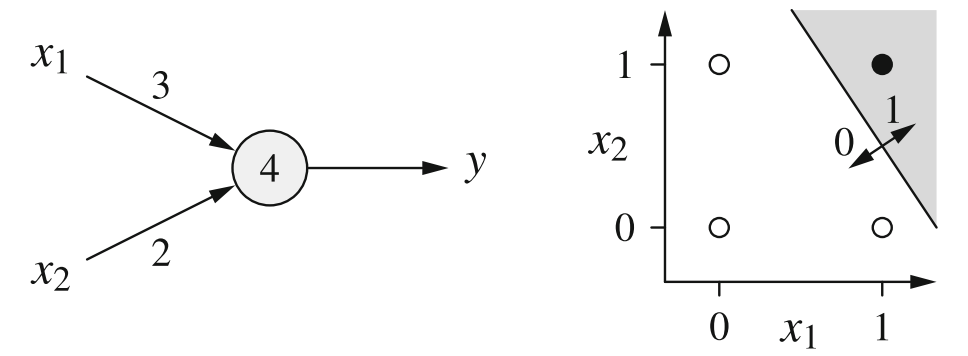
\includegraphics[scale=0.45]{images/geometric-tlu-and.png}
    \caption{Geometria dell'unità logica a soglia per $x1 \land x2$. La retta mostrata nel diagramma a destra ha l'equazione $3x1 + 2x2 = 4$; per il semipiano grigio, invece, è $3x1 + 2x2 \geq 4$.}
\end{figure}

\paragraph{Linearmente separabili}
Sappiamo dall'interpretazione geometrica delle loro computazioni che le Threshold Logic Unit possono rappresentare solo funzioni che sono, come si dice, \textit{linearmente separabili}, cioè funzioni per le quali i punti con output $1$ possono essere separati dai punti con output $0$ mediante una funzione lineare, ossia mediante una retta, un piano o un iperpiano.

Purtroppo, però, non tutte le funzioni sono linearmente separabili. Un esempio è la doppia implicazione, ossia $x1 \iff x2$. Due insiemi di punti $X$ e $Y$ si dicono linearmente separabili se e solo se i loro gusci convessi sono tra loro disgiunti.

\paragraph{Convesso}
Un insieme di punti $X$ in uno spazio euclideo si dice convesso se e solo se non è vuoto, è connesso e ogni coppia di punti può essere congiunta da un segmento

\paragraph{Convex hull}
Il più piccolo insieme convesso che contiene $X$

\paragraph{Doppia implicazione}
Non è possibile trovare pesi e una soglia tali che una TLU rappresenti la bi-implicazione. In generale, al crescere del numero di argomenti delle funzioni booleane, diminuisce il numero di funzioni che possono essere simulate da una singola Threshold Logic Unit. Tuttavia, è possibile costruire network di unità logiche a soglia per ovviare a questo problema

\paragraph{Networks of Threshold Logic Unit}
Il potere delle unità logiche a soglia è che, se le combiniamo insieme, possiamo risolvere alcuni compiti che una singola unità logica a soglia non può risolvere da sola. Consideriamo una possibile soluzione per il problema della bi-implicazione utilizzando tre unità logiche a soglia organizzate in due strati. Questa soluzione sfrutta l'equivalenza logica
$x1 \iff x2 \equiv (x1 \rightarrow x2) \land (x2 \rightarrow x1)$, che suddivide la doppia implicazione in tre funzioni. Sappiamo già che l'implicazione x2 → x1 è linearmente separabile.

\begin{figure}[h]
    \centering
    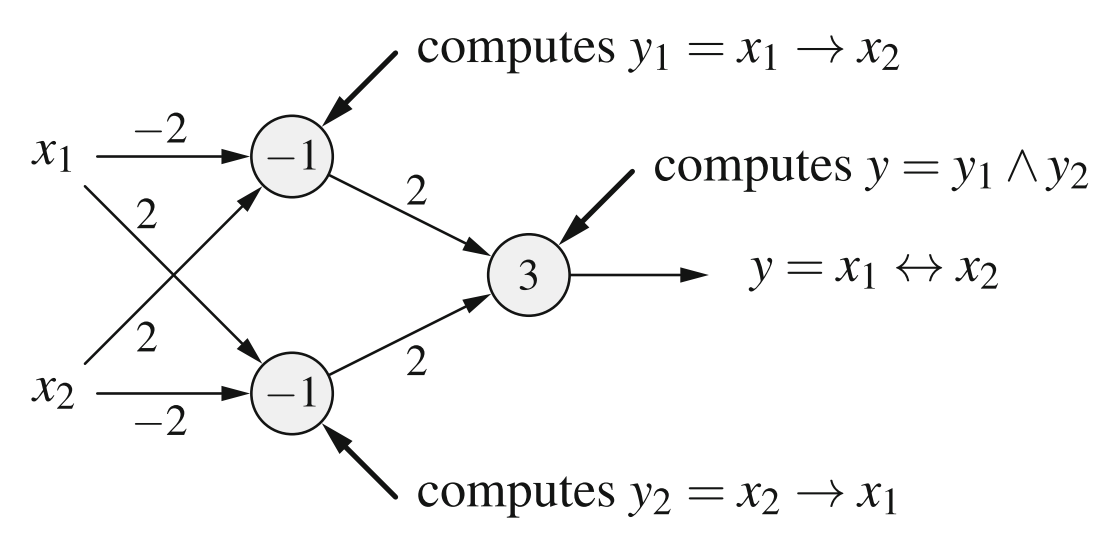
\includegraphics[scale=0.45]{images/tlu-bi-implicazione.png}
    \caption{Combina diverse unità logiche a soglia}
\end{figure}

La linea di separazione $g1$ corrisponde all'unità logica a soglia superiore e descrive l'implicazione $y1 = x1 \rightarrow x2$: per tutti i punti sopra questa linea l'output è $1$, per tutti i punti sotto di essa l'output è $0$. La linea di separazione $g2$ appartiene all'unità logica a soglia inferiore e descrive l'altra implicazione

\begin{figure}[h]
    \centering
    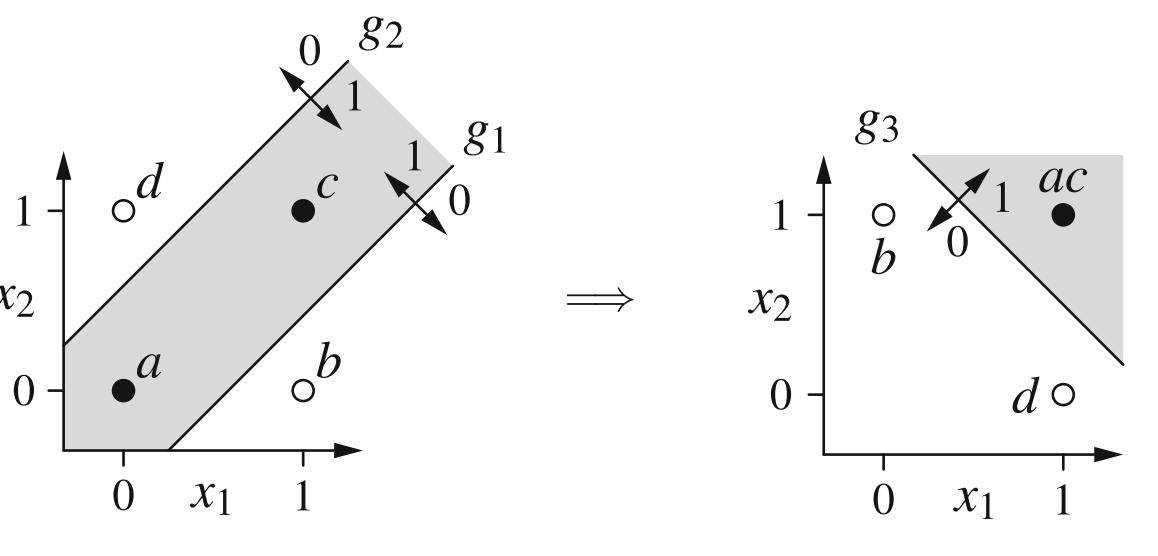
\includegraphics[scale=0.4]{images/geometric-tlu-bi-implication.png}
    \caption{Interpretazione geometrica della combinazione di più Threshold Logic Unit in una rete per calcolare la doppia implicazione}
\end{figure}

Tutte le funzioni booleane con input arbitrari possono essere calcolate utilizzando reti di unità logiche a soglia, sfruttando equivalenze logiche per suddividere le funzioni in sottofunzioni linearmente separabili.

\subsubsection{Training TLU}
La combinazione di più unità logiche a soglia in una rete per calcolare la doppia implicazione può essere interpretata geometricamente. Questo metodo funziona bene per funzioni con 2 o 3 variabili, in cui è possibile trovare facilmente una linea, un piano o un iperpiano che separi i punti per i quali l'output è 1 da quelli per cui l'output è 0. \uline{Dai parametri dell'equazione che descrive questa linea, piano o iperpiano, è possibile ricavare facilmente i pesi e la soglia}. Tuttavia, questo metodo diventa difficile e infine impossibile per funzioni con più di tre argomenti, poiché non siamo in grado di visualizzare lo spazio di input corrispondente. Inoltre, automatizzare questo metodo è impossibile poiché richiede una valutazione visiva dei set di punti da separare, un processo che non può essere replicato direttamente da un computer.

Per far evolvere una TLU in modo autonomo e automatizzato, possiamo utilizzare un algoritmo che procede nel seguente modo:
\begin{enumerate}
    \item Iniziamo assegnando valori randomici ai pesi e alla threshold
    \item Calcoliamo l'errore nell'output per un insieme di input di controllo. L'errore è una funzione dei pesi e della threshold, $e(w_1, \dots , w_n, \theta)$ che indica quanto bene, dati i pesi e la soglia, la funzione calcolata coincide con quella desiderata
    \item Aggiorniamo i pesi e la threshold in modo da correggere l'errore
    \item Iteriamo questo processo finché l'errore si annulla, ovvero finché l'output si avvicina il più possibile all'output desiderato
\end{enumerate}
L'algoritmo permette alla TLU di apprendere autonomamente, adattando i suoi pesi e il threshold per minimizzare l'errore nell'output. Questa lenta e graduale adattazione dei weights e della threshold (stepwise adaptation) viene anche chiamata learning/training. L'obiettivo è determinare quei valori in modo che la funzione abbia un errore pari a $0$. Per raggiungere questo obiettivo, cerchiamo di ridurre il valore della funzione di errore ad ogni passo.

\paragraph{Negazione booleana}
Nell'esempio considerato si vuole addestrare una TLU con un unico input, un unico peso associato, e un threshold per calcolare la negazione booleana. Sia $x$ l’input, $w$ il peso associato e $\theta$ la soglia, allora l’output $y$ sarà definito come:
$$
y = \begin{cases}
    1 & \text{se } 0w = 0 \geq \theta \\
    0 & \text{se } 1w = w \geq \theta
   \end{cases}
$$

\begin{figure}[h]
    \centering
    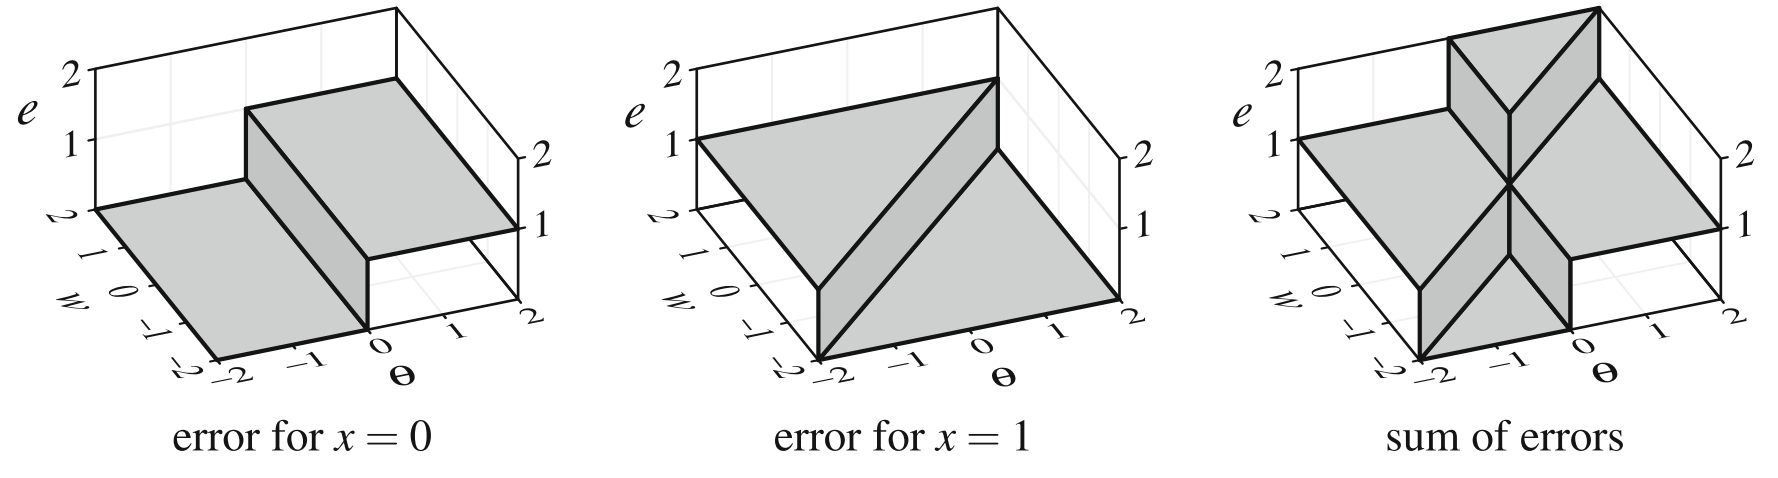
\includegraphics[scale=0.35]{images/error.png}
    \caption{Errore di calcolo della negazione rispetto alla soglia}
\end{figure}

La funzione di errore viene definita inizialmente come il valore assoluto della differenza tra l'output desiderato e l'output effettivo. Il diagramma a sinistra mostra l'errore per l'input $x = 0$, per il quale si desidera un output di $1$. Poiché la TLU calcola un $1$ se $xw \geq \theta$, l'errore è $0$ per una soglia negativa e $1$ per una soglia positiva. (Il peso non ha alcuna influenza, poiché viene moltiplicato per l'input, che è $0$).

Il diagramma centrale mostra l'errore per l'input $x = 1$, per il quale si desidera un output di $0$. Qui sia il peso che la soglia hanno un'influenza. Se il peso è inferiore alla soglia, abbiamo $xw \leq \theta$ e quindi l'output, e di conseguenza l'errore, è $0$. Il diagramma a destra mostra la somma di questi errori individuali.

Dal diagramma a destra, un essere umano può facilmente capire come scegliere il peso e la soglia in modo che la TLU calcoli la negazione: i valori di questi parametri devono trovarsi nel triangolo nella parte inferiore sinistra del piano $w-\theta$, in cui l'errore è $0$. L'adattamento automatico dei parametri utilizzando l'ispezione visiva della funzione di errore non è possibile direttamente con un computer. È necessario dedurre la direzione di modifica del peso e della soglia osservando la forma della funzione nell'attuale punto al fine di ridurre l'errore.

Per risolvere questo problema, modifichiamo la funzione di errore. Quando l'unità logica a soglia produce un output errato, consideriamo quanto il limite viene superato (per un output desiderato di $0$) o quanto viene sottoutilizzato (per un output desiderato di $1$). Intuitivamente, possiamo dire che il calcolo è "più sbagliato" quanto più il limite viene superato (exceeded) per un output desiderato di $0$, o quanto più viene sottoutilizzato (underrun) per un output desiderato di $1$.

Ci muoviamo semplicemente nella direzione in cui la funzione di errore ha la pendenza più ripida verso il basso. Cerchiamo cioè di \textit{descent in the error landscape}.

\begin{figure}[h]
    \centering
    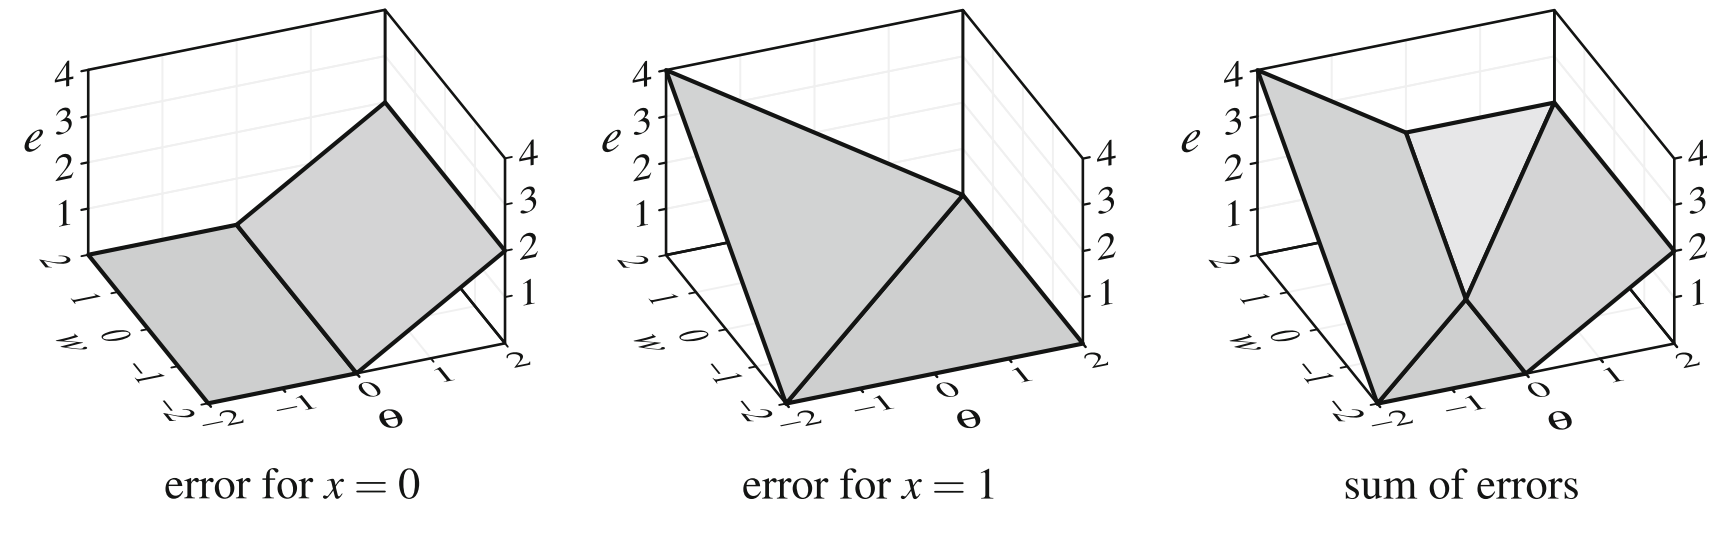
\includegraphics[scale=0.4]{images/error1.png}
    \caption{Funzione di errore differenziabile}
\end{figure}

\paragraph{Processo di allenamento} Ci sono due modi
\begin{itemize}
    \item \textit{Online learning}, correggiamo l’errore per ogni scelta dell’input
    \item \textit{Batch learning}, prendiamo in considerazione l’errore cumulato su una sequenza di input prima di applicare le correzioni
\end{itemize}

\paragraph{Delta rule o procedura di Widrow-Hoff}
Possiamo definire il seguente metodo generale di addestramento per le unità logiche a soglia.

Sia $\vec{v}$ = ($x_1, \dots, x_n$) il vettore di input di una TLU, $a$ l'output atteso e $y$ il valore attuale. Se $a$ = $y$, abbiamo finito. Al contrario, per ridurre l'errore computeremo nuovi valori per il threshold e i pesi nel seguente modo:
$$
\theta^{(new)} = \theta^{(old)} + \Delta\theta \text{ con } \Delta\theta = -\eta(a - y)
$$
$$
\forall i \in \{1, \dots, n\}:w_i^{(new)} = w_i^{(old)} + \Delta w_i \text{ con } \Delta w_i = \eta(a - y)x_i
$$
dove $\eta$ è il \textit{learning rate}\footnote{Parametro utilizzato negli algoritmi di apprendimento delle reti neurali che determina la dimensione dei passi di aggiornamento dei pesi durante il processo di adattamento del modello}. Più è alto, più i cambiamenti sui pesi e sui threshold sono elevati.

\uline{L'algoritmo utilizza la differenza tra l'output desiderato e l'output effettivo della rete per calcolare l'errore di predizione. Quindi, i pesi vengono aggiornati proporzionalmente a questo errore utilizzando un coefficiente di apprendimento. L'obiettivo è minimizzare l'errore di predizione adattando iterativamente i pesi della rete}.

\paragraph{Convergence Theorem for Delta Rule}
Esiste un teorema che ci garantisce che applicando la \textit{delta rule} l’algoritmo converge ad una soluzione.

Sia $L = \{(\vec{v_1},a_1), \dots, (\vec{v_n},a_n)\}$ una sequenza di pattern di allenamento per la TLU, dove $\vec{v_i}$ sono i vettori di input e $a_i$ l'output atteso. 
Siano inoltre $L_0 = \{(\vec{v},a) \in L | a = 0\}$ e $L_1 = \{(\vec{v},a) \in L | a = 1\}$ rispettivamente gli insiemi delle coppie di pattern che hanno come output atteso $0$ e quelle che hanno come pattern atteso $1$. Se $L_0$ e $L_1$ sono linearmente separabili, allora esiste un $\vec{w}$ vettore di pesi e un $\theta$ threshold t.c.:
$$
\forall (\vec{v},0) \in L_0: \vec{w}\vec{v} < \theta 
$$
$$
\forall (\vec{v},1) \in L_1: \vec{w}\vec{v} \geq \theta
$$

\paragraph{ADAptive LINear Element}
Nell'utilizzo delle Threshold Logic Unit per la risoluzione di problemi booleani, si è soliti rappresentare il valore falso come $0$ e il valore vero come $1$. Questo approccio può presentare un problema nel caso in cui il valore falso venga moltiplicato per un peso, poiché il risultato della moltiplicazione sarebbe sempre $0$ e non ci sarebbe modo di modificare il peso per correggere l'errore. Per ovviare a questo, si utilizza una diversa codifica chiamata ADALINE (ADAptive LINear Element), in cui falso viene rappresentato con il valore $-1$ e vero con $1$. Questo consente la modifica dei pesi anche in caso di valore falso.

È importante notare che la regola delta o la procedura Widrow-Hoff sono state originariamente sviluppate per il modello ADALINE (Widrow e Hoff 1960). Pertanto, possiamo correttamente riferirci a questa solo quando si utilizza il modello ADALINE.


%Artificial Neural Network
\subsection{Artificial Neural Network}
\paragraph{Grafo diretto}
Un grafo (orientato) è una coppia $G = (V, E)$ composta da un insieme (finale) $V$ di vertici o nodi e un insieme (finale) $E \subseteq V \times V$ di archi. Diciamo che un arco $e = (u, v) \in E$ è diretto dal vertice $u$ al vertice $v$

\uline{Per descrivere le reti neurali abbiamo bisogno solo di grafi orientati, poiché le connessioni tra i neuroni sono sempre dirette.}

\paragraph{Artificial neural network}
Una rete neurale artificiale è un grafo orientato $G = (U, C)$ i cui vertici $u \in U$ sono chiamati neuroni o unità e i cui archi $c \in C$ sono chiamati connessioni. L’insieme dei nodi $U$ può essere partizionato in tre sottoinsiemi
\begin{itemize}
    \item \textit{$U_{in}$}, nodi di input, ricevono l’informazione dall’ambiente
    \item \textit{$U_{out}$}, nodi di output, comunicano con l’esterno
    \item \textit{$U_{hidden}$}, nodi interni, propagano la computazione
\end{itemize}

\paragraph{Structure of neural networks}
Il grafo di una rete neurale viene spesso descritto da una matrice di adiacenza che, invece dei valori $1$ (connessione) e $0$ (nessuna connessione), contiene i pesi delle connessioni (se un peso è zero, la corrispondente connessione non esiste)

Questa matrice deve essere letta dall'alto verso destra: le colonne corrispondono ai neuroni da cui si originano le connessioni, le righe ai neuroni a cui le connessioni portano. Questa \uline{matrice e} il \uline{grafo pesato} corrispondente, ossia il grafo con archi pesati, \uline{sono chiamati struttura di rete}.

In base alla struttura di rete, possiamo distinguere due tipi fondamentali di reti neurali: se il grafo è aciclico, la rete viene chiamata \textit{\textbf{feed forward network}}, in questa rete i calcoli seguono di solito un ordinamento topologico\footnote{Un ordinamento topologico è una numerazione dei vertici di un grafo diretto, tale che tutti gli archi siano diretti da un vertice con un numero inferiore a un vertice con un numero superiore} dai neuroni di input progressivamente verso i neuroni di output. Se il grafo contiene cicli viene chiamata \textit{\textbf{recurrent network}}, in questo caso l'output finale può dipendere dall'ordine in cui i neuroni ricalcolano i loro output.

Ogni neurone possiede quattro variabili: 
\begin{enumerate}
    \item $net_u$, l'input totale che il neurone riceve dalla rete
    \item $act_u$, la funzione di attivazione applicata all'input
    \item $out_u$, l'output prodotto dal neurone dopo aver applicato la funzione di attivazione
    \item $ext_u$, eventuali input esterni al neurone
\end{enumerate}

\begin{figure}[h]
    \centering
    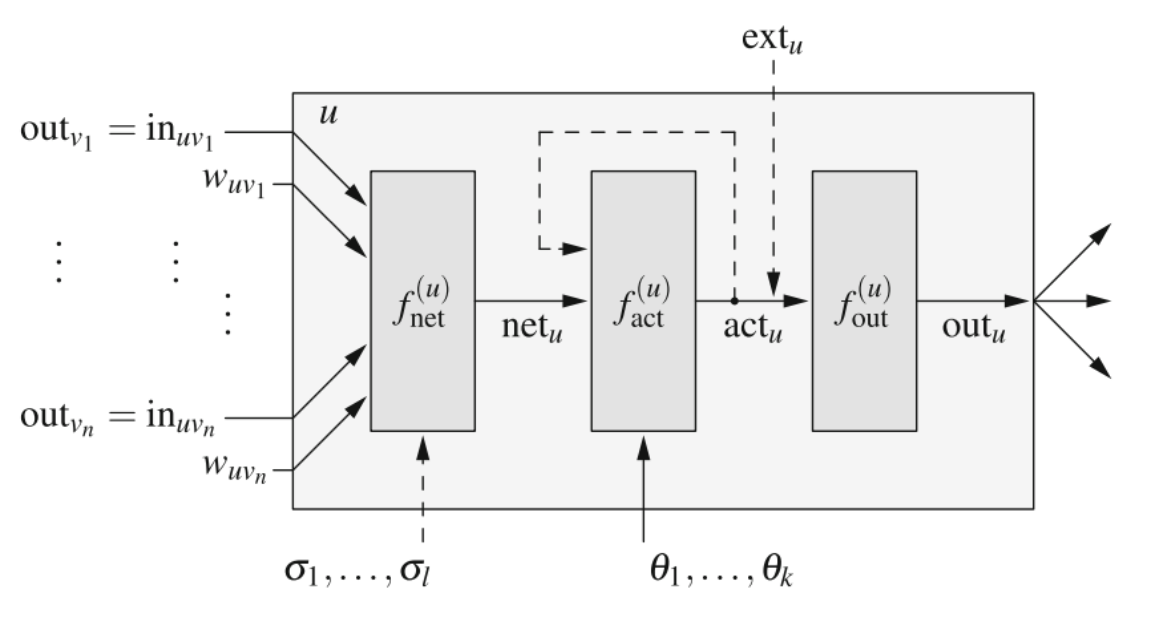
\includegraphics[scale=0.5]{images/structure_of_nn.png}
    \caption{Structure of Neural Network}
\end{figure}

Le prime tre variabili vengono calcolate in ogni momento dell’evoluzione dell’Artifical Neural Network grazie a tre funzioni associate
\begin{itemize}
    \item \textit{Network input function $f^u_{net}$}, calcola la somma pesata dell’input
    \item \textit{Activation funciont $f^u_{act}$}, vari modelli. Analizza l'input di rete dalla funzione precedente e genera lo stato di eccitazione del nostro neurone. Questo ci dirà se il neurone è sufficientemente eccitato.
    \item \textit{Output function $f^u_{out}$}, definisce l'output a seconda dell'attivazione del neurone. Prende lo stato di eccitazione del neurone e elabora lo stato finale del neurone per consegnarlo ai neuroni successivi
\end{itemize}

\paragraph{Processi interni}
Dividiamo i calcoli di una rete neurale in due fasi:
\begin{itemize}
    \item \textit{Input phase}, gli input esterni vengono acquisiti dai neuroni di input. Questa fase ha lo scopo di inizializzare la rete. Le attivazioni dei neuroni di input vengono impostate ai valori degli input esterni corrispondenti. Le attivazioni dei neuroni rimanenti vengono inizializzate arbitrariamente, di solito impostandole semplicemente a $0$. Inoltre, la funzione di output viene applicata alle attivazioni inizializzate, in modo che tutti i neuroni producano output iniziali. Se un neurone non riceve alcun input di rete perché non ha predecessori, viene definito che mantiene semplicemente la sua attivazione (e quindi anche il suo output).
    \item \textit{Work phase}, viene calcolato l'output della rete neurale. Cioè gli input esterni vengono disattivati e le attivazioni e gli output dei neuroni vengono ricalcolati (eventualmente più volte). I ricalcoli vengono interrotti se la rete raggiunge uno stato stabile, ovvero se ulteriori ricalcoli non modificano più gli output dei neuroni oppure se è stato effettuato un numero predeterminato di ricalcoli.
\end{itemize}

\subsubsection{Training Artificial Neural Network}
La delta rule ci consente di allenare automaticamente una singola TLU, questo non è generalizzabile alle ANN. Nonostante ciò, i principi su cui si basa la delta rule sono gli stessi utilizzati per allenare le Artificial Neural Network: calcolare le correzioni da applicare ai pesi e alla threshold dei singoli neuroni, aggiornandoli di conseguenza.
\paragraph{Tipi di apprendimento}
\begin{itemize}
    \item \textit{Fixed learning task}, supervisionato\\
    Avremo un insieme $L={(i_1, o_1), \dots , (i_n, o_n)}$ di coppie che assegnano ad ogni input un output desiderato. Una volta completato l'apprendimento, la ANN dovrebbe essere in grado di restituire l’output adeguato rispetto all’input presentato. In pratica, questo accade raramente e bisogna accontentarsi di un risultato approssimativo. Per giudicare in che misura una ANN si avvicina alla soluzione della fixed learning task si adotta una funzione di errore. Tale funzione viene calcolata come il quadrato della differenza tra l’output desiderato e quello attuale
    $$e = \sum_{l \in L} \sum_{v \in U_{(out)}} e^l_v \rightarrow e^l_v = (o^l_v - out_v)^2$$
    $e^l_v$ è l’errore individuale per una particolare coppia $l$ e un neurone di output $v$. La scelta di utilizzare il quadrato delle differenze come funzione di errore in primo luogo permette di tener conto degli errori positivi e negativi, evitando che si annullino a vicenda. In secondo luogo, questa funzione è ovunque derivabile, semplificando il processo di aggiornamento dei pesi e dei threshold, e consentendo di calcolare la direzione di miglioramento del modello in ogni punto.
    \item \textit{Free learning task}, non supervisionato\\
    Avremo solo una sequenza di input $L={i_1 , \dots , i_n }$. Non è possibile definire un output atteso per ogni input. In questo tipo di apprendimento l'obiettivo è quello di produrre un output simile per input simili, senza avere un output preciso da raggiungere.
\end{itemize}

\paragraph{Normalizzare il vettore di input}
Stiamo assumendo che gli input e gli output di una rete neurale siano numeri reali. Tuttavia, a volte i dati non sono in questa forma. Nella pratica, incontriamo attributi che hanno diversi tipi di scala, che possono richiedere una fase di pre-processing.

Comunemente lo si scala in modo tale che abbia media uguale a $0$ e varianza uguale a $1$. Per fare questo si calcola per ogni neurone $uk \in U_{in}$ la media aritmetica $\mu k$ e la deviazione standard $\sigma k$ degli input esterni

$$
\mu_k = \frac{1}{|L|}\sum_{l \in L} ext^l_{u_k} \quad \quad \sigma_k = \sqrt{\frac{1}{|L|}\sum_{l \in L} (ext^l_{u_k} - \mu_k)^2}
$$

%Multi-layer Perceptron
\subsection{Multi-layer Perceptron}
Le Multi-Layer Perceptron sono un tipo di rete neurale feed-forward composta da percettroni organizzati in diversi layer. Questa architettura prevede che ogni layer abbia connessioni solo con il layer successivo, garantendo così una struttura a flusso unidirezionale dell'informazione e riducendo le ricomputazioni durante la propagazione del segnale. I neuroni sono collegati in gruppi, ciascun gruppo riceve l'input solo dallo strato precedente o dall'input esterno. L'output viene inviato al gruppo successivo e ci sono diversi tipi di strati: strato di input, strato nascosto, strato di output. Le MLP rappresentano una delle prime tipologie di Artificial Neural Network sviluppate.

La network input function di ogni neurone nascosto e di ogni neurone di output $u \in U_{hidden} \cup U_{out}$ viene calcolata come la somma pesata (ponderata con i pesi delle connessioni) degli input:
$$
f^u_{net}(w_u,i_u) = \sum_{v \in pred(u)} w_{uv}out_v
$$
Nel caso delle Threshold Logic Units, abbiamo utilizzato la funzione a gradino come attivazione. Con i Multi-Layer Perceptron possiamo utilizzare funzioni sigmoide\footnote{Comunemente nei percettroni multistrato si utilizzano funzioni sigmoide, ma con gli sviluppi più recenti, come nel deep learning, vengono utilizzate diverse funzioni di attivazione. In particolare, la Rectified Linear Unit (ReLU).} come attivazione. Una {funzione sigmoide} è una funzione monotona non decrescente con:
$$
f: \mathbb{R} \to [0,1] \quad \text{ con } \lim_{x\to-\infty}f(x) = 0 \quad \text{ e } \lim_{x\to\infty}f(x) = 1
$$

Ha una forma che permette un valore minimo e massimo, in modo che lo stato netto possibile dei neuroni sia all'interno del dominio continuo tra $0$ e $1$ (questo è chiamato "squishification" dello stato della rete). Se ho abbastanza eccitazione nello stato della rete, la funzione sigmoide darà un'eccitazione positiva al neurone, viceversa, indicherà un valore più basso nella funzione. 

Ci sono molti tipi di funzioni sigmoide per rappresentare il comportamento generale, la più semplice è la funzione gradino. Ha un valore $0$ fino a quando l'eccitazione della rete raggiunge il valore $\Theta$, quindi l'uscita dell'eccitazione salta allo stato più forte (il valore di attivazione minimo e massimo è generalmente $0$ e $1$).

\begin{figure}[h]
    \centering
    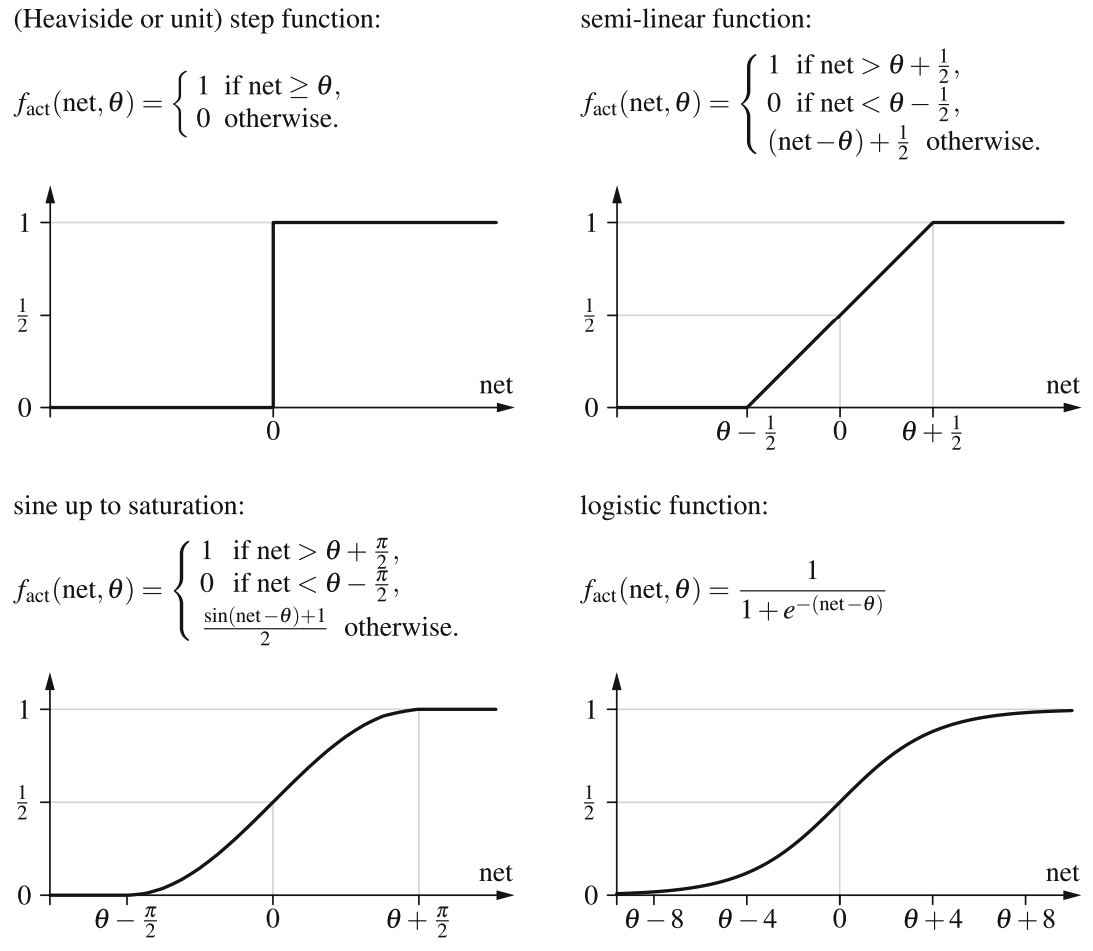
\includegraphics[scale=0.3]{images/fact.png}
\end{figure}

La funzione di output può essere una sigmoide o una funzione lineare. 

\paragraph{Matrice di peso: tutti i pesi tra due strati}
La struttura a layer suggerisce che il network possa essere descritto da una matrice dei pesi, semplificando la computazione attraverso la moltiplicazione tra matrici e vettori. Siano $U_1={v_1, \dots ,v_n}$ e $U_2={u_1, \dots ,u_m}$ due layer consecutivi di neuroni. I pesi delle loro connessioni sono codificati in una matrice $W$ di dimensioni $n \times m$:
\begin{center}$$
    W=\begin{pmatrix}
        w_{u_1v_1} & w_{u_1v_2} & \cdots & w_{u_1v_n} \\
        w_{u_2v_1} & w_{u_2v_2} & \cdots & w_{u_2v_n} \\
        \vdots & \vdots & \vdots & \vdots \\
        w_{u_mv_1} & w_{u_mv_2} & \cdots & w_{u_mv_n} \\
    \end{pmatrix}$$
\end{center}
Se due neuroni $u_i$ e $v_j$ non sono connessi, è sufficiente porre $w_{u_iv_j}=0$. Il vantaggio di questa matrice sta nel fatto che è possibile scrivere il network input di un layer come:
$$net_{U2}=w_{in_{U2}}=w_{out_{U1}}$$
dove $net_{U2}=(net_{u1},\dots,net_{um})^T$ e $in_{U2}=out_{U1}= (out_{v1},\dots,out_{vn})^T$

Basta prendere il vettore dei neuroni di input del secondo strato (che sono l'output dello strato precedente) e moltiplicarlo per il peso tra gli strati. Poi si applica la funzione sigmoide $\sigma$ per comprimere i valori tra $[0, 1]$,

%Function approximation
\subsubsection{Function approximation}
Capiamo cosa guadagniamo rispetto alle TLU, ovvero neuroni con la funzione di attivazione a gradino, se consentiamo l'utilizzo di altre funzioni di attivazione. Finora abbiamo visto funzioni booleane, ma ora vogliamo ampliare le dimensioni di una rete feed-forward per considerare non solo la funzione booleana dei TLU, ma vogliamo considerare in un perceptron multistrato qualsiasi tipo di numero reale (ampliare la capacità di descrivere il mondo). Il principio è
\begin{itemize}
    \item Approssimare una data funzione con una funzione a gradino
    \item Costruire una rete neurale che calcoli la funzione a gradino
    \item L'errore è misurato come l'area tra le funzioni
\end{itemize}

\begin{figure}[h]
    \centering
    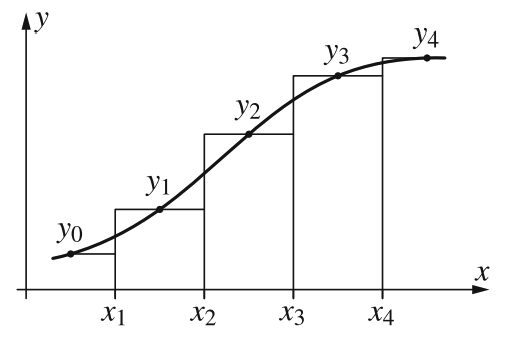
\includegraphics[scale=0.4]{images/step_function.png}
    \caption{Approssimare una funzione continua con funzioni a gradino. L'errore è l'area tra la funzione da approssimare e la step function}
    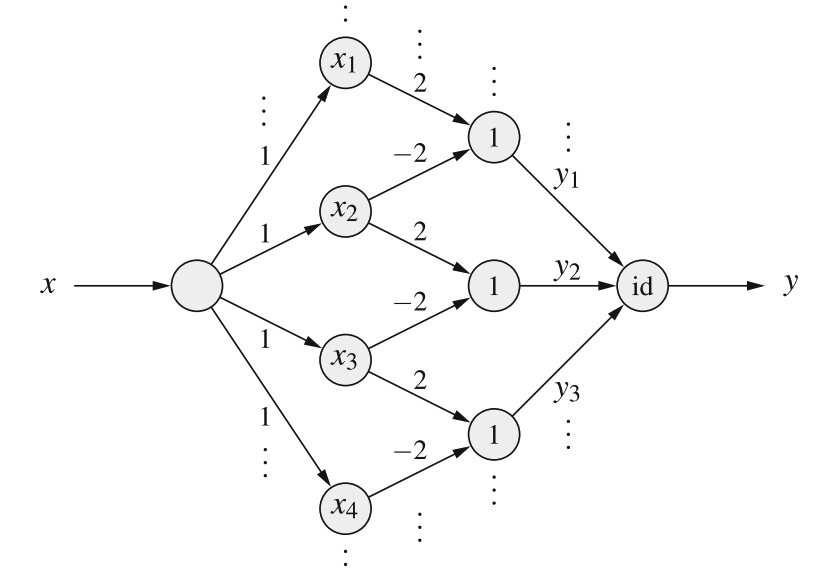
\includegraphics[scale=0.3]{images/mlp-step-function.png}
    \caption{Una rete neurale che calcola la funzione a gradino}
    \label{fig:enter-label}
\end{figure}

\begin{itemize}
    \item Per ogni valore di confine del gradino $x_i$, creiamo un neurone nel primo livello nascosto di un percettrone multistrato a quattro strati. Questo neurone serve a determinare da quale lato del valore di confine del gradino si trova il valore di input
    \item Nel secondo livello nascosto creiamo un neurone per ogni gradino, che riceve input dai due neuroni nel primo livello nascosto che si riferiscono ai valori $x_i$ e $x_i+1$ che segnano i confini di questo gradino. I pesi e la soglia sono scelti in modo tale che il neurone sia attivato se il valore di input non è inferiore a $x_i$, ma è inferiore a $x_i+1$, cioè se il valore di input si trova nell'intervallo del gradino. Si noti che in questo modo solo un neurone nel secondo livello nascosto può essere attivo, ovvero quello che rappresenta il gradino in cui si trova il valore di input
    \item Le connessioni dai neuroni del secondo livello nascosto al neurone di output sono ponderate con i valori della funzione dei gradini che sono rappresentati dai neuroni. Poiché solo un neurone può essere attivo nel secondo livello nascosto, il neurone di output riceve in input l'altezza del gradino in cui si trova il valore di input
\end{itemize}

Anche se l'errore di approssimazione può essere ridotto aumentando il numero di neuroni, ciò non garantisce che la differenza tra l'output del percettrone multistrato e la funzione da approssimare sia inferiore a un certo limite di errore in ogni punto. Questo perché potrebbero esserci picchi molto sottili nella funzione che non vengono catturati dai gradini. 

Non è la forma della funzione di attivazione, ma la struttura stratificata della rete feedforward che rende i percettroni multistrato approssimatori universali.

\paragraph{Delta approximation approach}
Possiamo effettivamente semplificare l'errore considerando un trucco invece di usare l'eccitazione combinata. Posso suddividere il dominio della funzione per la mia rete in parti come prima, quindi anziché definire il valore della funzione per ogni intervallo, utilizzo iterativamente la variazione $\Delta$ rispetto al valore considerato.

\begin{figure}[h]
    \centering
    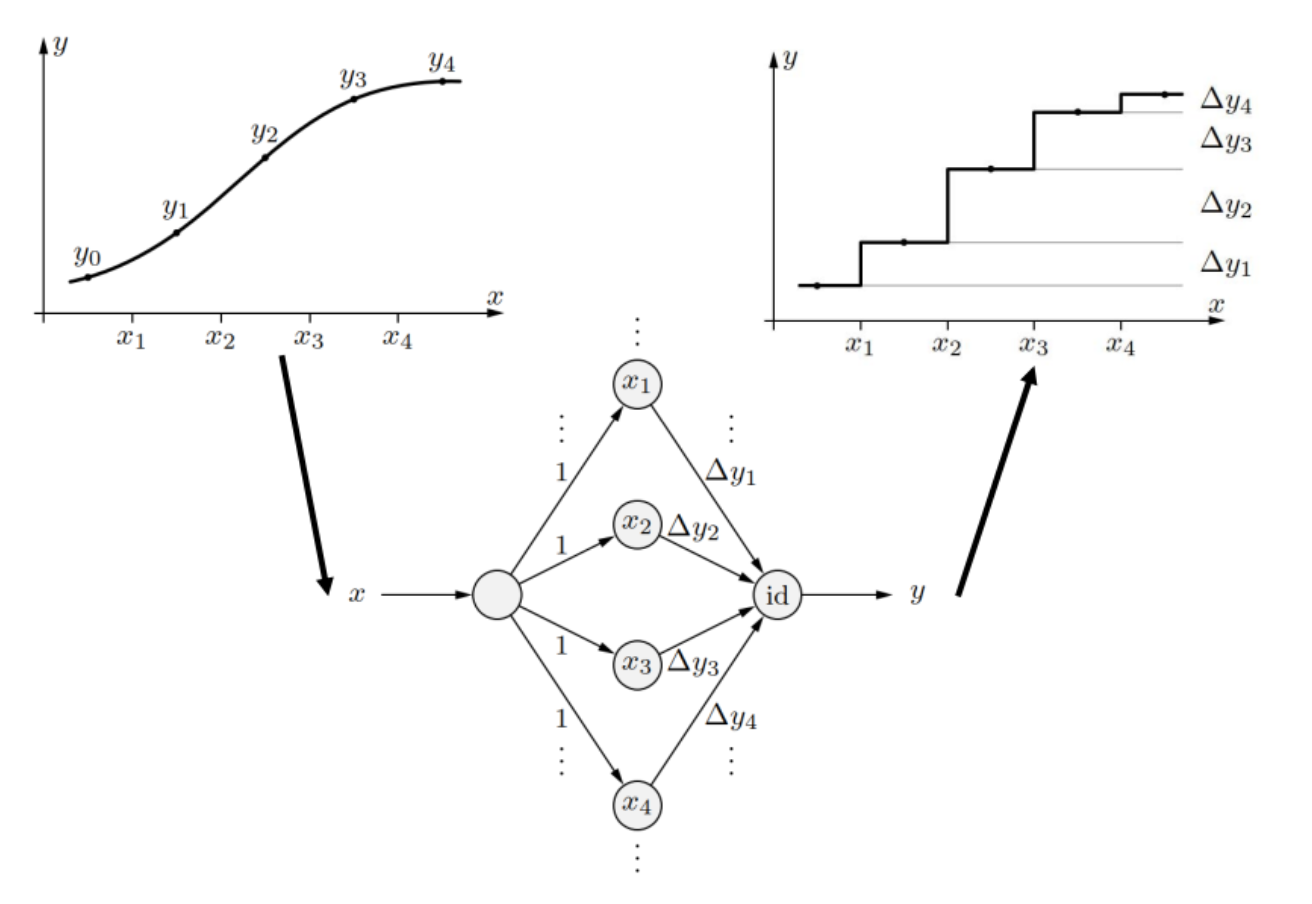
\includegraphics[scale=0.45]{images/delta_approximation_approach.png}
    \caption{Delta approximation approach}
\end{figure}

La struttura della rete sarà più semplice perché distribuirò l'input dei neuroni nascosti, che mi diranno se il valore $x$ è prima di $x_i$ o maggiore di $x_i$ (non mi interessa dove). Ad esempio, se il valore si trova tra $x_1$ e $x_2$, il primo neurone genererà $\Delta_{y1}$ e ciò sarà fornito in uscita. Se ho un valore compreso tra $x_2$ e $x_3$, avrò comunque $x_1$ che sarà abbastanza eccitato e genererà il contributo per l'output ($x_1$ e $x_2$ saranno entrambi eccitati, il loro contributo verrà sommato e quindi fornito in output). Questo renderà più semplice la struttura della rete.

\paragraph{Funzione Reimann}
Tutte le funzioni Reimann-integrabili possono essere approssimate con precisione arbitraria da percettroni a quattro strati, a condizione che il neurone di output abbia come funzione di attivazione l'identità invece di una funzione a gradino.

Questo teorema richiede solo che la funzione da rappresentare sia Riemann-integrabile, non è necessario che sia continua. In altre parole, la funzione da rappresentare può avere "salti". Tuttavia, può avere solo un numero finito di salti di altezza finita nella regione in cui deve essere approssimata. La funzione deve essere continua "quasi ovunque".

Il teorema mostra che i percettroni multistrato hanno elevata espressività ma nella pratica questo teorema ha scarso utilizzo. Per ottenere un'approssimazione accurata, infatti, richiede la creazione di MLP con un numero eccessivamente elevato di neuroni.


%Regressione
\subsection{Regressione}
Per allenare una rete neurale artificiale, si deve minimizzare la funzione di errore, che viene spesso calcolata come il quadrato della differenza tra l'output attuale e l'output atteso. Questo processo di apprendimento è simile al concetto più ampio di regressione utilizzato in analisi e statistica per estrarre la linea migliore (o, in generale, il polinomio) che approssima la relazione tra i dati di input e di output. La regressione ci aiuta a trovare i parametri della funzione che descrive meglio il dataset. \uline{A seconda del tipo di funzione che stiamo cercando di approssimare, esistono diverse forme di regressione}.

\subsubsection{Lineare}
Per ottenere una relazione lineare tra due variabili $x$ e $y$, è necessario trovare i parametri $a$ e $b$ che definiscono la retta $y = g(x) = a + bx$. Tuttavia, potrebbe non essere possibile trovare una singola retta che passi attraverso tutti i punti nel nostro dataset. Pertanto, utilizzeremo una tecnica di regressione per trovare la retta che si avvicina il più possibile ai punti nel dataset. Questo viene fatto minimizzando l'errore, che è calcolato come la somma dei quadrati delle differenze tra i valori predetti e i valori effettivi di $y$ per ogni punto nel dataset
$$F(a,b) = \sum(g(x_i) - y_i)^2 = \sum(abx_i - y_i)^2$$

\subsubsection{Polinomiale}
Il metodo precedente può essere esteso a polinomi di ordine arbitrario. In questo caso, si prende come ipotesi che la funzione indotta dal dataset approssimi un polinomio di ordine $n$
$$y = p(x) = a_o + a_1x + \dots + a_nx^n$$
E si cercherà di minimizzare la funzione $F$ tale che
$$ F(a_1,\dots,a_n) = \sum(p(x_i) - y_i)^2 = \sum(a_o + a_1x + \dots + a_nx^n -y_i)^2$$
Come nel caso della regressione lineare, la funzione potrà essere minimizzata solo se le derivate parziali rispetto ai parametri $a_i$ si annullano

\paragraph{Regressione multilineare}
E' possibile utilizzare la regressione per calcolare funzioni che dipendono da più di un parametro. L'idea di base rimane quella di trovare i parametri che minimizzano l'errore tra i valori attesi e quelli predetti.


\subsubsection{Logistica}
Quando ci troviamo in una situazione in cui la relazione tra le quantità nel nostro dataset non può essere approssimata con sufficiente precisione da una funzione polinomiale, potremmo dover utilizzare funzioni di altro tipo, ad esempio
$$y = ax^b$$
Possiamo trasformare questa funzione in una equazione lineare applicando il logaritmo naturale ad entrambi i membri dell'equazione
$$ln(y) = ln(a) + b \cdot ln(x)$$
Il motivo è che il calcolo di un polinomio di best fit può essere utilizzato anche per determinare altre funzioni di best fit. Nel caso delle Artificial Neural Network ci interessiamo in particolare alla funzione logistica
$$y = \frac{Y}{1 + e^{a+bx}}$$

dove $Y$, $a$ e $b$ sono costanti, esiste anche una trasformazione con la quale il problema può essere ridotto alla computazione di una linea di regressione, chiamata regressione logistica. La funzione logistica viene utilizzata molto frequentemente come funzione di attivazione.

\uline{Se una rete neurale utilizza come funzione di attivazione dei neuroni la funzione logistica, è possibile utilizzare il metodo della regressione per determinare i parametri della rete}. In particolare, si può applicare il metodo della regressione alla funzione logistica e ottenere i valori dei parametri $a$ e $b$. In questo modo, si possono determinare i parametri di qualsiasi rete a due layer con un singolo input. Il valore $a$ nella funzione corrisponderebbe alla threshold del neurone di output e la $b$ al peso dell’input

\paragraph{Logit transformation}
Se la \textit{$f^u_{act}$} è una logistica si può applicare la regressione per determinare i parametri della rete $a, b$. Dove $a$ è la treshold del neurone di output, e $b$ è il peso dell'input. Questo significa linearizzare la funzione logistica

Formiamo il valore reciproco dell'equazione logistica e prendiamo il logaritmo di questa equazione
$$y = \frac{Y}{1 + e^{a+bx}} \leftrightarrow \frac{1}{y} = \frac{1 + e^{a+bx}}{Y} \leftrightarrow \frac{Y - y}{y} = e^{a+bx} \leftrightarrow ln(\frac{Y - y}{y}) = a+bx$$

La somma degli errori quadratici può essere calcolata solo per i neuroni di output, limitando così l'uso di questo metodo ai percettroni a due strati, che hanno solo uno layer di input, uno di output senza hidden layer

%Backpropagation
\subsection{Backpropagation}
Concettualmente pensiamo che ogni neurone sia collegato a ogni neurone del livello precedente e la somma pesata di questi neuroni esprima la forza di tali connessioni:
$$\sigma(w_1u_1 + w_2u_2 + \dots w_nu_n + b)$$
Se consideriamo tutti i pesi e i bias inizializzati random, la rete MLP si comporterà piuttosto male perchè agirà casualmente. Quello che si fa è definire una funzione di costo che possa esprimere se il risultato della NN è buono o cattivo per il nostro obiettivo. Maggiore è il valore della funzione, maggiore è l'errore della NN rispetto all'output desiderato.
$$e_v^{(l)}=(o_v^{(l)} - out_v^{(l)})^2$$
Quindi, ciò che si fa è considerare la funzione di costo media su tutti gli esempi all'interno della NN. Vogliamo utilizzare questo errore in modo tale da poter eseguire meglio durante la prossima esecuzione, consideriamo una funzione $C(w)$ che rappresenta solo un costo, se vogliamo trovare l'input che minimizza il costo di questa funzione dobbiamo semplicemente prendere la derivata $dC(w) = 0$, ma ciò non è davvero praticabile per funzioni complesse. Si possono trovare diversi minimi locali della funzione, quindi ciò che si trova non è il valore di costo migliore possibile che si può trovare. Trovare il minimo globale è piuttosto difficile. La nostra funzione sarà molto più complicata, poiché stiamo lavorando con molti parametri (come i pesi e i bias), immaginiamo ora una funzione con due variabili in cui la funzione di costo è rappresentata graficamente come una superficie sopra il piano $xy$. Ora, per minimizzare la funzione, mi chiedo in quale direzione la funzione $C(x, y)$ diminuisce più rapidamente? Il calcolo multivariato ha un concetto di gradiente, che è la direzione dell'aumento più ripido $\vec{\nabla}C(x, y)$, e inoltre la lunghezza di quel vettore esprime quanto ripido è l'aumento. L'algoritmo sarà essenzialmente:
\begin{itemize}
    \item[I)] Calcola $\vec{\nabla}C(x, y)$
    \item[II)] Piccolo passo nella direzione $-\vec{\nabla}C(x, y)$
    \item[III)] Ripeti fino alla convergenza
\end{itemize}
Il gradiente negativo della funzione di costo ti dirà come cambiare tutti i pesi e i bias per tutte le connessioni, per ridurre efficientemente il costo.  La retropropagazione è un algoritmo per calcolare quel gradiente

%%Gradient descent
\subsubsection{Gradient descent}
Consideriamo il metodo della discesa del gradiente per determinare i parametri di un percettrone multistrato. Consiste nell'utilizzare la funzione di errore per calcolare la direzione in cui modificare i pesi e la threshold dei neuroni in modo da minimizzare l'errore complessivo della rete. Vogliamo trovare il minimo locale di una funzione di errore per trovare il giusto insieme di pesi

\begin{figure}[h]
    \centering
    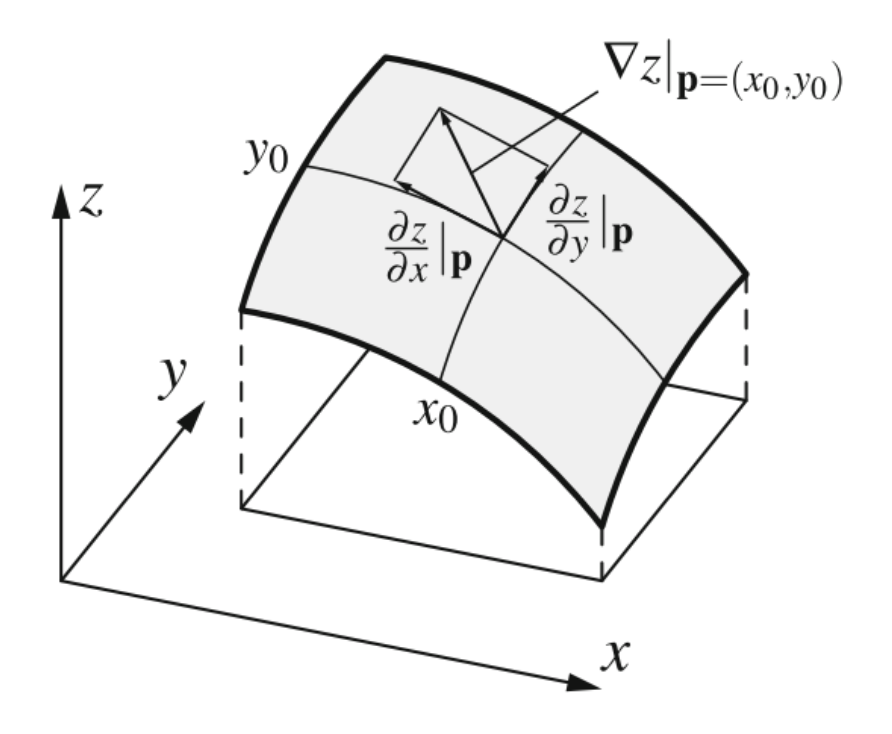
\includegraphics[scale=0.4]{images/gradient_descent.png}
    \caption{Interpretazione intuitiva del gradiente di una funzione a valori reali $z = f(x, y)$ in un punto $(x_0, y_0)$}
\end{figure}

Considerando questa superficie di errore in figura, se ci troviamo nel punto centrale possiamo osservare le derivate della funzione di errore nelle due direzioni, il gradiente $\nabla$ è il vettore tangente alla superficie che ci indicherà la direzione in cui la superficie sta aumentando o diminuendo di più. Se vogliamo trovare la soluzione per il nostro apprendimento, dobbiamo cercare il minimo di questa funzione di errore, quindi in realtà dobbiamo guardare nella direzione opposta al gradiente e cercare di raggiungere il minimo

Per poter utilizzare il gradient descent è necessario che la funzione di errore sia \textit{differenziabile}, ovvero che sia possibile calcolare la sua derivata in ogni punto. In questo modo, è possibile calcolare il gradiente della funzione di errore rispetto ai pesi e utilizzarlo per aggiornarli in modo iterativo fino a raggiungere un valore minimo di errore

\begin{enumerate}
    \item Inizializzazione dei pesi, assegnati casualmente
    \item Calcolo il gradiente della funzione di errore, rappresenta la direzione e l'entità del cambiamento necessario per ridurre l'errore della rete neurale
    \item Aggiornamento dei pesi, facendo un passo nella direzione opposta al gradiente, poiché vogliamo minimizzare l'errore, e aggiornando il learning rate che determina quanto i pesi vengono modificati ad ogni iterazione
    \item Ripetizione del processo, fino a quando l'errore della rete neurale viene ridotto a un livello accettabile o fino a quando viene raggiunto un numero massimo di iterazioni
\end{enumerate}

\paragraph{Gradiente} 
Il gradiente è un vettore espresso come n-dimensionale, dove n dipende dai pesi e dai bias, è di solito un numero enorme (impossibile da visualizzare). L'importante è che la magnitudine di ciascuna componente (quindi il valore) ti dirà quanto sensibile sarà l'output della funzione di costo rispetto al peso e al bias (quanto si sposta rispetto al valore precedente). Fondamentalmente, quando parliamo di addestramento o del processo di apprendimento di una NN, si tratta solo di minimizzare la funzione di costo, o funzione di errore.

Formalmente, il calcolo del gradiente restituisce un campo vettoriale. Ciò significa che il gradiente assegna a ogni punto del dominio della funzione un vettore, le cui componenti sono le derivate parziali della funzione rispetto ai suoi argomenti (conosciute anche come derivate direzionali). Questo vettore è spesso chiamato semplicemente il gradiente della funzione nel punto considerato. Punta nella direzione della pendenza più ripida della funzione in quel punto.

L'operatore differenziale $\nabla$ (chiamato nabla o del) viene utilizzato per calcolare il gradiente di un punto o di una funzione. \uline{Il principio è partire da un punto scelto casualmente nello spazio di ricerca, fare piccoli passi nello spazio dei parametri sempre nella direzione del massimo aumento (o diminuzione) della funzione da ottimizzare, fino a raggiungere un massimo o minimo locale, almeno approssimativamente}. Questa operazione consiste nell'identificare la direzione di massima pendenza (o variazione) in un dato punto, e quindi determinare la direzione in cui la funzione sta aumentando o diminuendo più rapidamente. Nel caso delle Multiple Layer Perceptron, calcolare il gradiente della funzione di errore si traduce nel \uline{calcolare la derivata parziale della funzione di errore rispetto ai pesi e i threshold presi come parametri}. Sia $w_u = (-\theta,w_{u_1},\dots,w_{u_k})$ il vettore dei pesi di un singolo layer esteso così da includere anche la threshold, calcoliamo il gradiente come segue
$$\nabla_{w_u} e = \frac{\partial e}{\partial w_u} = (-\frac{\partial e}{\partial \theta}, \frac{\partial e}{\partial w_{u_1}},\dots,\frac{\partial e}{\partial w_{u_k}})$$
Siccome l’errore totale $e$ è dato dalla somma degli errori individuali rispetto a
tutti i neuroni e tutti i training pattern $l$, otteniamo che
$$\nabla_{w_u} e = \frac{\partial e}{\partial w_u} = \frac{\partial}{\partial w_u} \sum_{l \in L} e^l = \sum_{l \in L} \frac{\partial e^l}{\partial w_u}$$

\paragraph{Error backpropagation}
Il processo che ci permette di calcolare la correzione necessaria per ogni peso e threshold di ogni singolo neurone dopo aver trovato l’errore. 

\uline{I valori di errore di ogni layer (nascosto) di un percettrone multistrato possono essere calcolati dai valori di errore del layer successivo. Possiamo anche dire che un segnale di errore viene trasmesso dall'output layer all'indietro attraverso gli hidden layer.}

\uline{Si assume che la funzione di attivazione sia la funzione logistica per ogni neurone $u \in U_{hidden} \cup U_{out}$ tranne che per quelli di input}.

\begin{enumerate}
    \item \textit{Setting the input}, applichiamo l’input ai neuroni di input che lo restituiscono senza modifiche in output al primo dei layer hidden
    \item \textit{Forward propagation of the input}, calcolare per ogni neurone dei livelli successivi la somma pesata degli input e applicare al risultato la funzione logistica, producendo l'output che sarà propagato in tutta la rete fino ai neuroni terminali.
    \item \textit{Error factor}, calcoliamo la differenza tra l'output atteso e quello attuale. Utilizzando l'inversa della funzione di attivazione, possiamo risalire all'input che ha causato quell'errore
    \item \textit{Error backpropagation}, trasformiamo l'errore dell'output in un errore dell'input possiamo distribuire l'errore (con la correzione) in modo proporzionale indietro al neurone precedente, propagando l'errore fino ai neuroni di input.
\end{enumerate}
L'adattamento dei pesi viene eseguito mediante la seguente formula (che mi dice come eseguire la correzione):
$$\forall w_{up} : \sigma w_{up} = \eta\sigma_u out_p$$

\paragraph{Variazioni gradient descent}
Uno dei problemi che possiamo incontrare è il "rimanere bloccati" in un minimo locale. Esistono varie sofisticazioni della tecnica del gradient descent che permettono un più veloce apprendimento
\begin{itemize}
    \item[I)] \textit{Manhattan training}, utilizza al posto del valore del gradiente solo il segno per calcolare la direzione. E' veloce ma non riesce ad ottenere l'ottimo
    \item[II)] \textit{Flat spot elimination}, è una tecnica utilizzata per affrontare il problema dei plateau, ovvero delle zone in cui la funzione di attivazione del neurone ha una derivata molto bassa o addirittura nulla. Quando ci si avvicina a un plateau, l'abbattimento della lunghezza degli step di apprendimento può limitare notevolmente l'efficienza dell'aggiornamento dei pesi. Per ovviare a questo problema, la tecnica del flat spot elimination solleva artificialmente la derivata della funzione di attivazione nel punto in cui la derivata è molto bassa, in modo da evitare che la lunghezza degli step di apprendimento si abbatta troppo. Questo sollevamento viene fatto aggiungendo un valore costante alla funzione di attivazione nel punto in cui la derivata è bassa.
    \item[III)] \textit{Momentum term}, viene aggiunto un termine che rappresenta la memoria del passato del cambiamento dei pesi. E' utile perché in molte situazioni il gradiente può avere una grande variazione tra le iterazioni e può essere instabile, quindi l'aggiunta di questo termine può aiutare a mantenere una direzione coerente per il cambiamento dei pesi
    \item[IV)] \textit{Self-Adaptive Error backpropagation: SuperSAB}, aggiunge un termine di adattamento ai learning rate dei singoli parametri. Il tasso di apprendimento di ogni parametro viene adattato in base al suo gradiente locale. Se il gradiente è grande, viene ridotto, in modo da limitare il rischio di oscillazioni indesiderate. Al contrario, se il gradiente è piccolo, il tasso di apprendimento viene aumentato, in modo da favorire il rapido apprendimento.
    \item[V)] \textit{Resilient error backpropagation}, combina il manhattan training con il self-adaptive
    \item[VI)] \textit{Quick propagation}, al posto di utilizzare il gradiente approssimo la fun- zione con una parabola e salto direttamente all’apice della parabola. Se la funzione di errore è "benigna", il training può avvicinarsi molto al minimo effettivo in un singolo passo di allenamento.
    \item[VII)] \textit{Weight decay}, 
    tecnica utilizzata per evitare una crescita eccessiva dei pesi con conseguente overfitting del modello
\end{itemize}

\paragraph{Cross validation}
Per capire se abbiamo una buona qualità per il nostro apprendimento, dobbiamo dividere casualmente i nostri set di dati in due parti: training set; validation set. Possiamo fare la suddivisione in due modi:
\begin{itemize}
    \item \textit{Cross validation}, divide casualmente i dati in due sottoinsiemi, addestriamo l'MLP con diversi numeri di neuroni nascosti sui dati di addestramento e li valutiamo sui dati di convalida. Quindi ripetiamo la suddivisione dei dati, l'addestramento e la valutazione molte volte e facciamo la media dei risultati. Alla fine scegliamo il numero di neuroni nascosti con l'errore medio migliore.
    \item \textit{k-fold cross validation}, i dati vengono divisi in $k$ sottoinsiemi di dimensioni uguali. Di questi $k$ sottoinsiemi, vengono formati $k$ coppie di set di dati di addestramento e convalida utilizzando $1$ fold come convalida e $k - 1$ fold per l'addestramento. Il campione viene suddiviso in gruppi di uguale dimensione, un gruppo alla volta viene escluso per verificare la bontà del modello di previsione utilizzato. Interrompiamo l'addestramento quando l'errore di convalida è sufficientemente basso
\end{itemize}

%Overfitting e underfitting
\subsubsection{Overfitting e underfitting}
Di quanti neuroni ho bisogno per avere un buon network? Come regola di massima si dovrebbe scegliere il numero di neuroni negli hidden layer secondo la seguente formula:
$$\mathit{hidden\;neurons} = \frac{input\;neurons + output\;neurons}{2}$$
Il numero di neuroni negli hidden layer deve essere valutato in modo da evitare l'\textit{underfitting} o l'\textit{overfitting}. Un numero troppo basso di neuroni può portare ad un modello insufficientemente complesso, mentre un numero troppo elevato può far sì che il modello si adatti troppo ai dati di training, generando un'alta varianza e quindi un alto errore di generalizzazione. Per questo motivo, è importante dividere il dataset in due sottoinsiemi: training set e validation set. In questo modo, si può valutare l'accuratezza del modello su dati mai visti durante il processo di apprendimento e scegliere il numero ottimale di neuroni negli hidden layer per minimizzare l'errore di generalizzazione.

\subsubsection{Sensitivity analysis}
Le Artificial Neural Network presentano uno svantaggio in termini di comprensione della conoscenza acquisita durante il processo di apprendimento. Questa viene rappresentata in matrici a valori reali che risultano di difficile interpretazione per l'utente. Esiste un'interpretazione geometrica dei processi interni alle ANN ma offre poco aiuto all'intuizione quando lo spazio degli input supera le tre dimensioni. Per superare questo problema, una soluzione è quella di eseguire una \textit{sensitivity analysis}, che determinerà l'influenza dei vari input sull'output del network. Per eseguirla, occorre \uline{calcolare la somma delle derivate parziali degli output rispetto agli input esterni per ogni neurone di output e ogni training pattern. Questa somma viene infine divisa per il numero di training pattern}, per rendere la misura indipendente dalla grandezza del dataset.
$$\forall u \in U_{(in)}: \quad s(u) = \frac{1}{|L|} \sum_{l \in L} \sum_{\nu \in U_{(out)}} \frac{\partial out_\nu^l}{\partial ext_u^l}$$
Il valore $s(u)$ indica quanto importante fosse l’input assegnato al neurone $u$ per la computazione del Multi-Layer Perceptron. Potremmo decidere di semplificare il network eliminando i nodi con i valori di $s(u)$ più bassi.

%Deep learning
\subsection{Deep learning}
La rete di apprendimento profondo è essenzialmente un MLP, ma con una differenza: ciò che vogliamo fare è non avere alcun tipo di conoscenza sul problema e cercare di forzare la NN a configurarsi con un numero limitato e piccolo di neuroni. 

La formula di Reinmann ha mostrato come un MLP con un solo hidden layer può approssimare ogni funzione continua su $\mathbb{R}^n$ con una precisione arbitraria. Può non essere semplice conoscere a priori il numero esatto di neuroni necessari per approssimare una data funzione. Inoltre, a seconda della funzione, questo numero potrebbe assumere dimensioni considerevoli. 

Un esempio è quello della funzione che calcola la parità su una parola di n-bit. L’output sarà $1$ se e solo se nel vettore di input che rappresenta la parola saranno ad $1$ un numero pari di bit. Nel caso scegliessimo di utilizzare un Multi-Layer Perceptron con un solo hidden layer questo avrà al suo interno $2^{n-1}$ neuroni, in quanto la forma normale disgiuntiva della funzione di parità su n-bit è una disgiunzione di $2^{n-1}$ congiunzioni. 

\uline{L'utilizzo di più di un hidden layer promette di ridurre il numero di neuroni necessari}. \uline{Questo è il focus dell'area del deep learning}, dove la "profondità" di una rete neurale è quella che separa i neuroni di input da quelli di output. Una maggiore profondità del network in cambio di un miglioramento delle risorse utilizzate nel calcolo e nella costruzione. Il deep learning oltre ad offrire vantaggi porta con se alcune problematiche: \textit{Overfitting}, l'aumento dei neuroni dati dagli ulteriori layer nascosti può moltiplicare i parametri in modo sproporzionato; \textit{Vanishing gradient}

\paragraph{Soluzioni overfitting}
\begin{itemize}
    \item \textit{Weigth decay}, limita i valori che possono assumere i pesi della rete neurale, ponendo un tetto massimo alla grandezza dei pesi. In pratica, durante l'addestramento, viene aggiunto un termine alla funzione di costo che penalizza i pesi più grandi, in modo che i pesi non raggiungano valori troppo elevati.
    \item \textit{Sparsity constraint}, limite al numero di neuroni negli hidden layer, oppure limite sul numero di quelli attivi
    \item \textit{Dropout training}, alcuni neuroni degli hidden layer vengono omessi durante l’evoluzione del network
\end{itemize}

%Vanishing gradient
\subsubsection{Vanishing gradient}
Il vanishing gradient è un problema che si verifica in una rete neurale \uline{quando il gradiente utilizzato nell'algoritmo di backpropagation dell'errore diminuisce significativamente in valore man mano che ci si avvicina ai primi layer della rete}. Questo problema si verifica spesso nelle reti neurali con funzioni di attivazione non lineari e derivate che assumono valori compresi tra $0$ e $1$. Nel caso della funzione di attivazione logistica, la sua derivata raggiunge al massimo il valore di $\frac{1}{4}$. Quando il gradiente diventa molto piccolo, l'aggiornamento dei pesi diventa meno efficace, e quindi la rete neurale impiega più tempo per apprendere e può anche avere difficoltà a convergere

\paragraph{Modificare la funzione di attivazione}
Una soluzione è quella di modificare leggermente la funzione di attivazione in modo che sia sempre crescente. Alcuni candidati proposti in letteratura sono la \textit{ramp function} e la \textit{softplus function}

\paragraph{Autoencoder}
Un approccio completamente diverso consiste nel costruire il perceptron multistrato strato per strato, addestrando solo il nuovo strato aggiunto in ogni passaggio. Una procedura molto popolare per fare ciò è costruire la rete come \textit{stacked autoencoder}. \uline{Un autoencoder è un perceptron multistrato che mappa i suoi input in un'approssimazione di questi input, utilizzando un hidden layer}.

Lo strato nascosto (e le connessioni che lo collegano allo strato di input) forma un encoder che trasforma gli input in una forma di rappresentazione interna, che viene poi decodificata dallo strato di output (e dalle connessioni dallo strato nascosto allo strato di output). Un tale autoencoder viene addestrato con la back-propagation standard, o una delle sue varianti, che non soffre molto del problema del vanishing gradient, poiché c'è solo uno strato nascosto.

\begin{enumerate}
    \item \textit{Sparse autoencoder}, prevede di utilizzare un numero molto minore di neuroni nell'hidden layer, rispetto a quelli di input in  modo che l'autoencoder sia costretto ad imparare alcune caratteristiche effettivamente rilevanti invece di propagare solo i dati.
    \item \textit{Sparse activation scheme}, disattivare casualmente alcuni neuroni durante la fase di calcolo
    \item \textit{Denoising autoencoder}, si aggiunge rumore all’input
\end{enumerate}

\paragraph{Layer-wise training: addestramento strato per strato} Per costruire un MLP con molti strati, è possibile utilizzare una tecnica chiamata layer-wise training. Inizialmente si allena un autoencoder con un singolo strato nascosto utilizzando la backpropagation per minimizzare l'errore di ricostruzione tra l'input e l'output dell'autoencoder. Una volta addestrato, il decoder dell'autoencoder viene rimosso e viene conservato solo il layer nascosto, che viene utilizzato come input per l'addestramento di un nuovo autoencoder con un altro strato nascosto. Questo processo viene ripetuto fino a raggiungere il numero desiderato di strati nascosti.

Questa tecnica è stata utilizzata con successo per la classificazione di immagini, ad esempio nel riconoscimento di numeri scritti a mano. Tuttavia, per applicazioni più complesse in cui le feature da riconoscere non sono localizzate in una specifica parte dell'immagine, sono necessarie architetture più avanzate come le Convolutional Neural Network (CNN).

\paragraph{Convolutional Neural Network}
\uline{Questo tipo di rete è ispirato alla struttura della retina umana, in cui i neuroni sensoriali hanno un cosiddetto campo recettivo, cioè una regione limitata in cui rispondono a uno stimolo visivo}. Questo viene imitato in una CNN connettendo ogni neurone nello strato nascosto (primo) solo a un piccolo numero di neuroni di input contigui (nell'immagine). I pesi della rete sono condivisi tra le diverse regioni, in modo che la stessa feature possa essere rilevata in posizioni diverse dell'immagine. \uline{Durante la computazione, il campo ricettivo viene spostato su tutta l'immagine e viene eseguita una convoluzione tra la matrice dei pesi e l'immagine in input per produrre una mappa delle feature}. Questa mappa viene quindi sottoposta ad un pooling, ovvero ad una riduzione della dimensione, per ridurre la complessità del modello e prevenire l'overfitting. Questo processo viene ripetuto per tutti gli strati nascosti della rete fino a raggiungere l'output finale.

%Radial Basis Function Network
\subsection{Radial Basis Function Network}
Le RBFN hanno diversi use cases, come function approximation, time series prediction, classificazione. E' strettamente limitata ad avere un solo strato nascosto, che chiamiamo \textit{feature vector}. L'input layer si limita a ricevere i dati di ingresso e feedarli nell'hidden layer, il calcolo che avviene nello strato nascosto è molto diverso da quello della maggior parte delle reti neurali. Lo strato di output esegue operazioni di previsione come classificazione o regressione.

\begin{itemize}
    \item \textit{Input layer}: i neuroni sono completamente connessi con lo strato nascosto, non fanno nessuna computazione ma solo feeding dei dati
    \item \textit{Hidden layer}: prende in input un modello che potrebbe non essere linearmente separabile e lo trasforma in un nuovo spazio più linearmente separabile, per questo il numero di neuroni è maggiore rispetto a quello di input per il teorema di Cover
    \item \textit{Outuput layer}: funzione di attivazione lineare
\end{itemize}

I Radial Basis Function Network sono reti neurali feed-forward con tre layer di neuroni, questo significa che c'è esattamente un layer nascosto. \uline{Rispetto ai Multi-Layer Perceptron, hanno una funzione di attivazione diversa, chiamata funzione radiale di base.} Nei neuroni di output, la somma pesata degli input avviene come nei MLP. Nel layer nascosto, invece, la funzione \textit{net} è una funzione di distanza tra il vettore di input e il vettore dei pesi. Questa distanza deve rispettare tre assiomi geometrici per essere considerata una metrica.
$$d(w,v) = 0 \leftrightarrow w = v \mathit{\;\;(equality)}$$
$$d(w,v) = d(v,w) \mathit{\;\;(simmetry)}$$
$$d(w,e) + d(e,v) \geq d(w,v) \mathit{\;\;(triangle\;inequality)}$$
La funzione di input della rete per i neuroni di output è la somma pesata degli input.
La funzione di attivazione di ogni neurone nascosto è una funzione radiale.
La funzione di attivazione di ogni neurone di output è una funzione lineare.
La funzione di input di rete e le funzioni di attivazione di un neurone nascosto descrivono una sorta di "zona di influenza" di questo neurone. I pesi delle connessioni dallo strato di input a un neurone dello strato nascosto indicano il centro di questa regione, poiché la distanza (funzione di input di rete) viene misurata tra il vettore dei pesi e il vettore di input. Il tipo di funzione di distanza determina la forma della zona di influenza

\begin{figure}[h]
    \centering
    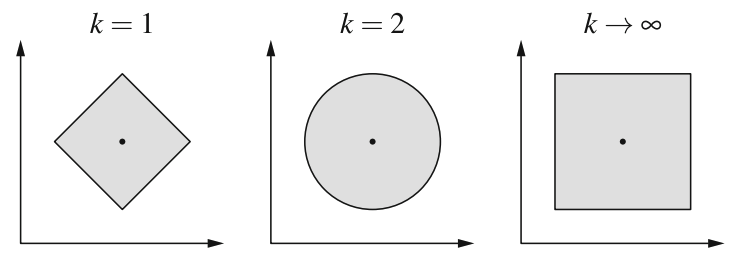
\includegraphics[scale=0.4]{images/rbfn.png}
    \caption{Cerchi per diverse funzioni di distanza. Tutti i cerchi hanno lo stesso raggio.}
\end{figure}

In modo intuitivo, la funzione di attivazione di un hidden neuron e i suoi parametri determinano la "dimensione" della zona di influenza del neurone specificando quanto sia forte l'influenza di un vettore di input in base alla sua distanza dal vettore dei pesi. Chiamiamo questa funzione di attivazione una funzione radiale, perché è definita lungo un raggio da un centro, che è descritto dal vettore dei pesi e assegna a ciascun raggio (cioè, a ciascuna distanza dal centro) un'attivazione.

Una famiglia di funzioni usate spesso nelle applicazioni è quella formulata dal matematico Minkowski e rinominata in suo onore famiglia di Minkowski. Tale famiglia è definita come
$$d(w,v)_k = (\sum (w_i - v_i)^k)^{\frac{1}{k}}$$
Alcune funzioni appartenenti alla famiglia
$$k = 1: \mathit{Manhattan\;distance}$$
$$k=2:\mathit{Euclidian\;distance}$$
$$k = \infty: \mathit{Maximum\;distance, ovvero\;} d(w,v)_\infty = max |w_i - v_i|$$

La funzione di attivazione di ciascun hidden neuron è una funzione radiale cioè una funzione monotona non crescente
$$f: \mathbb{R}^{+} \to [0,1] \quad \mathit{con} \quad f(0) = 1 \quad \mathit{e} \quad \lim_{x \to \infty} f(x) = 0$$
Questa funzione calcola l’area in cui il neurone focalizza la propria attenzione definita dal raggio di riferimento $\sigma$.


\paragraph{Approximation functions}
Un RBFN ha la capacità di approssimare funzioni con un errore arbitrariamente piccolo, allo stesso modo di un MLP, e quindi può essere considerato come un \uline{approssimatore universale}. Questo significa che \uline{può approssimare qualsiasi funzione Riemann-integrabile}.

%Learning Vector quantization
\subsection{Learning Vector quantization}
LVQ è un algoritmo di classificazione supervisionato basato su prototipi. E' un precursore delle Self-Organizing Maps (SOM). Addestra la sua rete attraverso un algoritmo di Competitive Learning simile alla Self-Organizing Map

Fino ad ora abbiamo descritto l'apprendimento delle Aritificial Neural Network in relazione ai fixed learning task, dove l'obiettivo è di adattare la rete per approssimare gli output desiderati per un determinato insieme di input. Tuttavia, ci sono situazioni in cui non siamo in grado di conoscere gli output desiderati per tutti i nostri dati in ingresso. In questi casi, l'obiettivo della rete neurale può essere quello di raggruppare o classificare i dati in modo automatico, senza alcuna indicazione su quale sia l'obiettivo specifico. Una tecnica che aiuta nel \uline{clustering automatico dei dati} è la Learning Vector Quantization.

Quantizzazione vettoriale dell'apprendimento (Kohonen $1986$). L'obiettivo di questo metodo è organizzare i dati in cluster, i singoli cluster sono rappresentati da un centro. Questo centro viene posizionato in modo che si trovi approssimativamente al centro del gruppo di punti dati che costituisce il cluster.

\subsubsection{Vector quantization network}
La learning vector quantization utilizza una rete feed-forward a due layer chiamata Learning Vector Quantization Network (LVQN). Questa rete può essere vista come una variante della Radio Basis Function Network, in cui il layer di output sostituisce il layer nascosto. Come nelle RBFN, la funzione di input del layer di output dipende dalla distanza tra il vettore di input e i pesi associati ai neuroni e la funzione di attivazione dei neuroni di output è una funzione radiale. 

La differenza principale rispetto alle RBFN è che la $f_{(out)}$ non è l'identità, ma viene propagata solo se l'attivazione del neurone è la massima tra tutti i neuroni di output. 

\paragraph{Winners takes all}
Il neurone con la maggiore attivazione produce l'output $1$, tutti gli altri neuroni producono output $0$

\paragraph{Competitive learning}
L'apprendimento competitivo nella LVQ comporta la competizione tra i neuroni di output per attivarsi in risposta a un punto di input, con il neurone vincitore che viene adattato per avvicinarsi al punto e gli altri neuroni che vengono spinti lontano. Questo processo si ripete per ogni punto di input nel dataset, consentendo alla rete neurale di adattare i suoi vettori di riferimento per una migliore rappresentazione dei dati di input

\paragraph{Attraction rule}
Sposta il vettore di riferimento verso il punto di input
$$r^{new} = r^{old} + \eta(x - r^{old})$$

\paragraph{Repulsion rule}
Sposta gli altri vettori di riferimento associati ai neuroni non vincenti lontano dal punto di input
$$r^{new} = r^{old} - \eta(x - r^{old})$$
dove $x$ è l’input, $r$ è il vettore di riferimento per il neurone vincitore e $\eta$ è il learning rate

\begin{figure}[h]
    \centering
    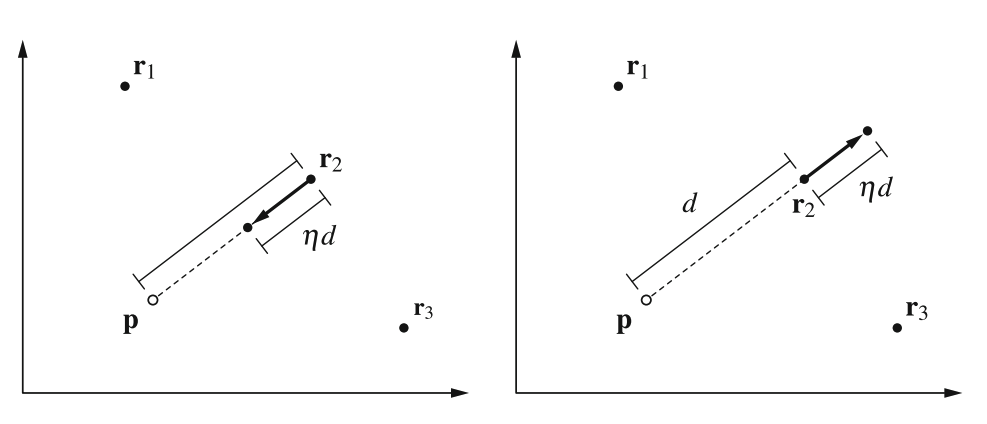
\includegraphics[scale=0.35]{images/attraction-repulsion.png}
    \caption{Sinistra attraction rule, destra repulsion rule}
\end{figure}

Dopo la competizione, i vettori di riferimento associati al neurone vincente vengono adattati in modo che il vettore di riferimento sia mosso più vicino al punto di input, mentre gli altri vettori di riferimento associati ai neuroni non vincenti vengono allontanati dal punto

\paragraph{Time dependent learning rate}
Finora abbiamo dato per scontato che $\eta$ rimanesse costante durante l'intero processo di apprendimento, ma ci sono alcune situazioni in cui un tasso di apprendimento costante può causare problemi. Infatti, se è troppo elevato, la rete neurale potrebbe oscillare attorno al punto di ottimizzazione senza mai raggiungerlo, mentre se è troppo basso, l'apprendimento potrebbe essere troppo lento e richiedere molto tempo per convergere verso un minimo globale

Per risolvere il problema del $\eta$ costante, un metodo è quello di far decrescere il learning rate al crescere delle iterazioni. In questo modo, il movimento circolare collassa col passare del tempo in una spirale, facendo così convergere l’algoritmo

\begin{figure}[h]
    \centering
    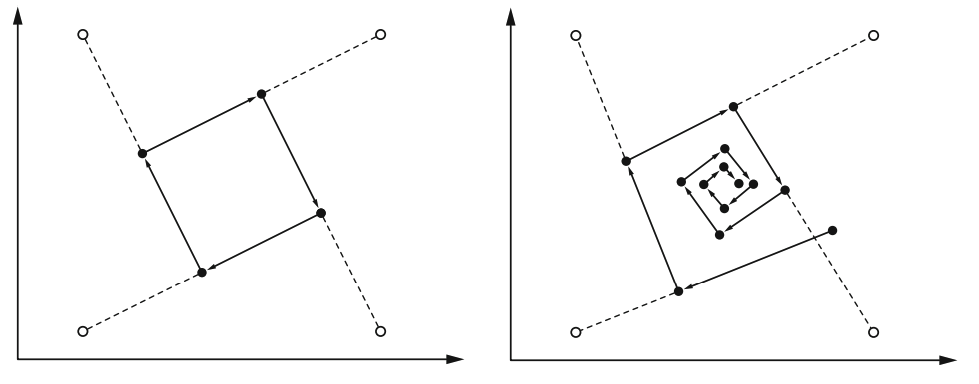
\includegraphics[scale=0.35]{images/dependent-learning-rate.png}
    \caption{Learning rate costante a sinistra, decrescente a destra}
\end{figure}

%Self-organizing maps
\subsection{Self-organizing maps}
Una Self-Organizing Map è una tecnica di apprendimento automatico non supervisionato utilizzata per produrre una rappresentazione a bassa dimensione (tipicamente bi o tri dimensionale) di un insieme di dati di dimensioni più elevate, preservando la struttura topologica dei dati. 
E' un tipo di ANN trainata utilizzando competitive learning invece della back-propagation con il gradient descent. Come la maggior parte delle reti neurali artificali, operano in due modalità:
\begin{itemize}
    \item \textit{Training}, utilizza un insieme di dati di input (input space) per generare una rappresentazione a bassa dimensione (map space)
    \item \textit{Mapping}, classifica ulteriori dati di input utilizzando la mappatura generata
\end{itemize}

Le SOM, o mappe delle caratteristiche di Kohonen, sono strettamente correlate alle Radial Basis Function Network. \uline{Possono essere considerate reti a funzione di base radiale senza uno strato di output, o, più precisamente, l'hidden layer di una Radial Basis Function Network è già lo strato di output di una Self-Organizing Maps}. I neuroni sono disposti in una griglia.

Una SOM è una rete neurale a due strati senza hidden neuron. La sua struttura corrisponde essenzialmente allo strato di input e allo strato nascosto delle Radial Function Base Network

Le self-organizing maps, o \textit{mappe delle caratteristiche di Kohonen}, sono una tipologia di rete neurale feed-forward a due strati che possono essere considerate come una generalizzazione delle Learning Vector Quantization. A differenza di quest'ultime, le connessioni tra i neuroni nascosti e quelli di output sono limitate solo ai neuroni "vicini". In pratica, ogni neurone di output è associato a un'area della mappa bidimensionale e, durante la fase di apprendimento, i neuroni della mappa vengono organizzati in modo tale da riflettere la struttura dei dati in input. In questo modo, i neuroni della mappa vicini a quelli attivati da un particolare input si attivano anch'essi, formando una sorta di cluster o regione di attivazione. Le SOM possono essere utilizzate per la visualizzazione dei dati, la classificazione e la riduzione della dimensionalità.

La funzione di output di ciascun neurone di output è l'identità. L'output può essere discretizzato secondo il principio del \textit{winners takes all}.

Come nel caso dei LVQN, la $f_{(net)}$ dei neuroni di output è una funzione di distanza tra il vettore di input e quello dei pesi, e la $f_{(act)}$ è una funzione radiale\footnote{Funzione che restituisce un valore basato sulla distanza tra l'input e un centro specifico nello spazio}.

Sui neuroni dello strato di output è definita una relazione di vicinato, descritta da una funzione di distanza
$$d_{\text{neurons}} : U_{\text{out}} \times U_{\text{out}} \rightarrow \mathbb{R}^{+}$$
Questa funzione assegna un numero reale non negativo a ciascuna coppia di neuroni di output.

\begin{figure}[h]
    \centering
    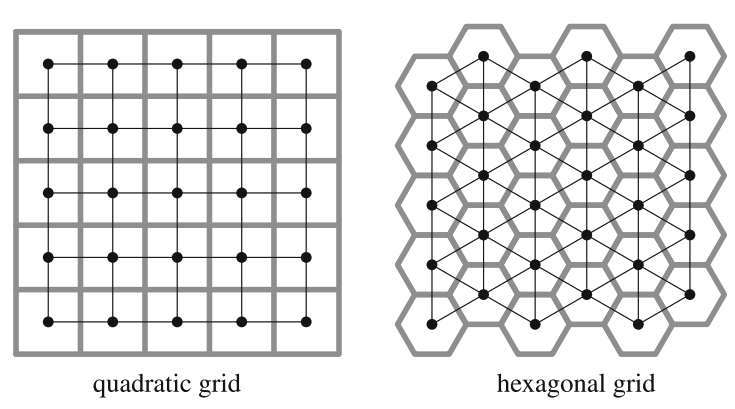
\includegraphics[scale=0.4]{images/som-structure.png}
    \caption{Esempi di disposizioni dei neuroni di output di una Self-Organizing Map. Ogni punto corrisponde a un neurone di output. Le linee sono intese per rendere più chiara la struttura di vicinato}
\end{figure}

In analogia alle reti a funzione di base radiale, nelle mappe auto-organizzanti i pesi delle connessioni dall'input ai neuroni di output rappresentano le coordinate di un centro, chiamato \textit{reference vector}, rispetto al quale viene misurata la distanza di un pattern di input. Più un pattern di input si avvicina al vettore di riferimento, maggiore sarà l'attivazione del neurone corrispondente. Questo significa che il neurone di output che ha il vettore di riferimento più simile al pattern di input avrà un'attivazione più alta rispetto agli altri neuroni di output.

Quando si parla di quantizzazione vettoriale dello spazio di input, si intende che la mappa auto-organizzante suddivide lo spazio di input in diverse regioni, ognuna delle quali è associata a un neurone di output. Ogni regione rappresenta un insieme di input simili che sono mappati sul neurone di output corrispondente. Quindi, la mappa auto-organizzante consente di raggruppare i pattern di input in base alle loro caratteristiche simili, creando una rappresentazione compressa dello spazio di input.

\paragraph{Proiezioni di Robinson}
\uline{La self-organizing map è una funzione che preserva la topologia, cioè conserva la posizione relativa tra i punti del dominio}. Un esempio di funzione che preserva la topologia sono le proiezioni di Robinson, utilizzate per costruire le mappe del globo. Queste proiezioni conservano la posizione relativa tra i punti anche se la proporzione della distanza tra due punti nell'originale e nella proiezione è maggiore quanto più ci si allontana dall'equatore. \uline{Utilizzando queste funzioni, è possibile mappare spazi multidimensionali in spazi con dimensioni minori, offrendo un vantaggio in termini di efficienza computazionale}.

Applicato alle Self-Organizing Maps, i punti di intersezione delle linee della griglia sulla sfera potrebbero indicare la posizione dei vettori di riferimento nello spazio di input, mentre i punti di intersezione delle linee della griglia nella proiezione indicano la posizione dei neuroni di output e la loro relazione di vicinato.

\paragraph{Competitive training}
\uline{Nelle SOM, l'apprendimento si basa sul competitive training}, dove ogni input viene assegnato al neurone con l'attivazione più alta. Non solo il neurone vincitore viene aggiornato, ma anche i suoi vicini, sebbene in misura minore. Questo evita che i vettori di riferimento dei neuroni vicini si muovano arbitrariamente lontani l'uno dall'altro, mantenendo così la topologia dello spazio di input. La regola di apprendimento utilizzata per trovare la corretta funzione che preservi tale topologia è una \textit{generalizzazione della attraction rule}.
$$r^{new} = r^{old} + \eta(t)f_{nb}(d_{neuroni}(u,u_*),\rho(t))(x - r^{old})$$
dove $u_*$ è il neurone vincitore e $f_{nb}$ è una funzione radiale. Il learning rate $\eta$ è parametrizzato rispetto al tempo perché varierà con il numero delle iterazioni


%Hopfield network
\subsection{Hopfield network}
E' un tipo di rete neurale artificiale nota per essere il modello di rete che simula le capacità del cervello umano di ricordare le cose o di ricostruire le immagini distorte. Questo modello è classificato come apprendimento non supervisionato, la rete impara senza avere esempi, soltanto con l'uso del concetto di \textit{energia}.

In precedenza ci siamo concentrati esclusivamente sui modelli di reti neurali feed-forward, ovvero modelli di reti neurali rappresentati da grafi aciclici. Tuttavia, esistono anche modelli di \textit{recurrent network}, il cui grafo di connessione presenta dei cicli diretti. Tra questi, uno dei modelli più semplici è quello degli Hopfield Network, che ha avuto origine come modelli fisici per descrivere il magnetismo. Rispetto agli altri tipi di Artifial Neural Network, gli HN presentano alcune differenze: \uline{tutti i neuroni sono contemporaneamente neuroni di input e di output, non ci sono hidden neuron e ogni neurone è connesso con tutti gli altri neuroni (sono eslusi cappi) con pesi di connessione simmetrici}. 

La rete può essere rappresentata come un grafo completamente connesso, con pesi simmetrici tra i neuroni e archi a loop con peso $0$. Poiché lo strato di input e lo strato di output sono fusi nello stesso strato, il numero di input e output della rete è uguale al numero di neuroni.

La funzione di input di ogni neurone è determinata dalla somma pesata degli output degli altri neuroni.
$$f_{(net)}^u(w,i) = \sum_{v \in U - \{u\}} w_{uv} out_v $$
La funzione di attivazione è una threshold function
$$
f_{(act)}^u(net_u,\theta_u) = 
    \begin{cases}
	1 \quad \text{se} \quad net_u >= \theta_u \\
        -1 \quad \text{se} \quad net_u < \theta_u
    \end{cases}
$$
Possiamo rappresentare un Hopfield Network attraverso la sua matrice dei pesi che contiene la forza delle connessioni tra i neuroni, visto che i neuroni non si connettono a se stessi, i pesi sulla diagonale sono nulli.
$$
W = \begin{bmatrix} 
        0 & w_{u_1 u_2} & \dots & w_{u_1 u_n} \\
        w_{u_2 u_1} & 0 & \dots & w_{u_2 u_n} \\
        \vdots & \vdots & \vdots & \vdots \\
        w_{u_n u_1} & w_{u_n u_2} & \dots & 0
     \end{bmatrix}
$$

La funzione di output è la funzione identità. Per ogni neurone, l'output viene calcolato con una funzione che confronta la somma pesata degli input con la soglia e restituirà $1$ se il valore è superiore o uguale alla soglia, altrimenti $0$. Il problema di questo tipo di rete è che l'output di ogni neurone si diffonde a tutti gli altri neuroni: se l'aggiornamento dello stato viene fatto parallelamente, non sarà possibile garantire uno stato finale stabile della rete, ma cambierà continuamente. La soluzione è eseguirlo sequenzialmente (considerando il teorema di convergenza) e convergerà a uno stato finale in al massimo $n\cdot2^n$ passaggi.

\paragraph{Teorema convergenza}
Se i neuroni di un HN sono aggiornati in modo asincrono allora uno stato stabile viene raggiunto al massimo in $n\cdot 2^n$ passi, dove $n$ è il numero dei neuroni. La prova del teorema si basa sul calcolo dell'energia del sistema
$$E = -\frac{1}{2} \sum_{u,v \in U, u \neq v} w_{uv}act_u act_v + \sum_{u \in U} \theta_u act_u$$
Gli HN sono in grado di raggiungere uno stato stabile che corrisponde ad un minimo locale della funzione energia del sistema. Ciò significa che il network può solo evolvere verso uno stato con energia minore rispetto a quello attuale. Questo fatto può essere sfruttato per utilizzare gli HN come \textit{memorie associative}, dove si collega un dato allo stato stabile raggiunto dopo averlo processato attraverso il network. Inoltre, gli HN possono essere impiegati per risolvere \textit{problemi di ottimizzazione}, dove la ricerca della soluzione ottimale corrisponde alla ricerca del minimo globale della funzione energia del sistema

\paragraph{Use cases}
\begin{itemize}
    \item Memoria associativa, un esempio è la nostra capacità di riconoscere un'immagine anche quando questa non è esatta o riconosere un vecchio amico rivedendolo dopo anni. La memoria associativa è un sistema in cui il richiamo della memoria è avviato dall'associabilità di un modello di input a uno memorizzato. Questo ci permette di recuperare e completare un ricordo utilizzando solo una parte incompleta o rumorosa di esso
    \item Risoluzione di problemi di ottimizzazione
    \item Simulated annealing, è un'evoluzione del gradiente che accetta di esplorare soluzioni che sono peggiori di quella corrente, permettendo di sfuggire agli ottimi locali. Con una rete di Hopfield questa tecnica viene implementata controllando, per ogni transizione di stato, se lo stato raggiunto avrà un'energia più bassa o più alta. Nel primo caso, la transizione viene sempre accettata perché descrive una soluzione migliore, nel secondo caso la transizione viene accettata solo con una certa probabilità proporzionale al peggioramento dell'energia che sarebbe ottenuto.
\end{itemize}

%Boltzmann machines
\subsection{Boltzmann machines}
Le macchine di Boltzmann sono simili alle Hopfield Network in quanto entrambi utilizzano una funzione energia associata ad ogni stato per risolvere problemi di ottimizzazione. Tuttavia, le macchine di Boltzmann sono più complesse, poiché possono contenere hidden neuron e hanno una procedura di aggiornamento differente. 

In questa fase di aggiornamento viene selezionato casualmente un neurone e, con i suoi input, vengono calcolati i delta di energia con cui viene calcolata la probabilità di attivazione. Questa procedura viene ripetuta diverse volte selezionando casualmente i neuroni. Alla fine degli aggiornamenti, lo stato finale è indipendente dallo stato iniziale e dai neuroni iniziali aggiornati, e questo stato finale è chiamato Equilibrio Termico.

La procedura di aggiornamento descritta sopra non è sempre utilizzabile:
\begin{itemize}
    \item È computazionalmente pesante e quindi non è applicabile a reti di grandi dimensioni
    \item Funziona bene con dati distribuiti secondo una distribuzione di Boltzmann, ma non così bene con altre distribuzioni. Una soluzione a questo problema è utilizzare la cosiddetta "Restricted Boltzmann Machine" 
\end{itemize}

\uline{La funzione energia viene utilizzata per definire una distribuzione di probabilità (di Boltzmann) rispetto agli stati del network}
$$P(\overrightarrow{s}) = \frac{1}{c} e^{-\frac{E(\overrightarrow{s})}{kT}}$$
dove $s$ è l'insieme degli stati, $c$ una costante di normalizzazione, $E$ la funzione energia, $T$ la temperatura del sistema, $k$ la costante di Boltzmann ($k \simeq 1,38 \cdot 10^{-23}$).
I possibili valori di attivazione dei neuroni all'interno del sistema rappresentano gli stati del sistema stesso. \uline{Per definire la distribuzione di probabilità associata ai vari stati del sistema, si utilizza una funzione energia}. La probabilità di attivazione di un neurone viene calcolata utilizzando una funzione logistica, la quale tiene conto della differenza di energia tra il caso in cui il neurone è attivo e quello in cui è inattivo.
$$P(act_u = 1) = \frac{1}{1 + e^{-\frac{\Delta E_u}{kT}}}$$
dove 
$$\Delta E_u = E_{act_u = 1} - E_{act_u = 0} = \sum_{v \in U - \{u\}} w_{uv} act_v - \theta_u$$

\paragraph{Markov-chain Monte Carlo}
E' la procedura di aggiornamento che prevede di scegliere randomicamente un neurone e calcolare il suo differenziale energetico e, con questo, la probabilità di attivazione. Questa stessa procedura viene ripetuta varie volte fino alla convergenza del sistema

\subsubsection{Training Boltzmann machines}
L'obiettivo dell'apprendimento in una macchina di Boltzmann è quello di adattare i pesi delle connessioni tra i neuroni e i loro threshold in modo tale che la distribuzione di probabilità implicita nel dataset di addestramento sia approssimata dalla distribuzione rappresentata dai neuroni visibili della BM. Per fare ciò, si definisce una funzione di costo che descrive la differenza tra le due distribuzioni e si utilizza la tecnica del \textit{gradient descent} per minimizzarla

\paragraph{Kullback-Leibler}
$$KL(p1,p2) = \sum_{\omega \in \Omega} p1(\omega) ln\frac{p1(\omega)}{p2(\omega)}$$
dove $p1$ si riferisce alla distribuzione del dataset e $p2$ a quella della macchina di Boltzmann. Ogni passo di apprendimento viene suddiviso in due fasi
\begin{enumerate}
    \item \textit{Positive phase}
    \item \textit{Negative phase}
\end{enumerate}
Se distinguiamo la probabilità che un neurone $u$ sia attivato nella positive phase $p_u^{+}$ e quella che lo stesso neurone sia attivato nella negative phase $p_u^{-}$ e la probabilità che due neuroni $u$ e $v$ siano attivati simultaneamente nella positive phase $p_{uv}^{+}$ e quella che gli stessi due neuroni siano attivati nella negative phase $p_{uv}^{-}$, possiamo definire la regola di update dei pesi e della threshold
$$\Delta w_{uv} = \frac{1}{\eta} (p_{uv}^{+} - p_{uv}^{-}) \quad \mathit{e}\quad\Delta \theta_u = -\frac{1}{\eta}(p_u^{+} - p_u^{-})$$
Se un neurone viene sempre attivato quando viene presentato lo stesso input, il suo threshold verrà ridotto. Allo stesso modo, se due neuroni vengono spesso attivati assieme, il peso della loro connessione verrà aumentato 

\subsubsection{Restricted Boltzmann machines}
Non ammettono connessioni intra-layer, cioè non c'è connessione tra unità visibili-visibili e tra unità nascoste-nascoste.

Le restricted Boltzmann machines sono state introdotte per ridurre il dispendio di risorse necessario per allenare le BM di dimensioni medie. \uline{La differenza principale tra una RBM e una BM classica è che il grafo del network di una RBM è bipartito}. I neuroni sono essenzialmente bipartiti in neuroni visibili e nascosti. I neuroni visibili sono quelli che ricevono l'input esterno e sono completamente connessi solo con i neuroni nascosti, i neuroni nascosti prendono in input l'output dei neuroni visibili e sono completamente connessi solo con loro. 

Grazie a questa struttura, il processo di apprendimento di una RBM può essere svolto in modo efficiente attraverso tre passaggi
\begin{enumerate}
    \item Le unità di input vengono fissate rispetto ad un pattern scelto casualmente e quelle nascoste vengono aggiornate in parallelo ottenendo quello che si chiama \textit{positive gradient}
    \item Si invertono le parti, si fissano i neuroni nascosti e si aggiornano quelli visibili, ottenendo il \textit{negative gradient}
    \item Si aggiornano pesi e threshold con la differenza tra positive e negative gradient
\end{enumerate}

%Recurrent network
\subsection{Recurrent network}
Sia gli Hopfield Network che le Boltzmann Machines sono esempi di recurrent network. \uline{In questi network, l'output viene prodotto solo quando il sistema raggiunge uno stato stabile nella sua elaborazione}.

\paragraph{Training}
Questa rete può essere addestrata con una backpropagation modificata che gestisce i loop.

\paragraph{Use cases}
Rappresentazione di sistemi di equazioni differenziali.\\
La dinamica di questi sistemi può essere descritta attraverso l'utilizzo di \textit{equazioni differenziali}, che vengono rappresentate in forma ricorsiva. 
$$x(t_i) = x(t_{i-1}) + \Delta y_1(t_{i-1})$$
$$y_1(t_i) = y_1(t_{i-1}) + \Delta y_2(t_{i-1})$$
$$\vdots$$
$$y_{i-1}(t_i) = y_{i-1}(t_{i-1}) + f(t_{i-1}, x(t_{i-1}), \dots, y_{n-1}(t_{i-1}))$$

Queste equazioni possono essere utilizzate per calcolare il valore successivo di una variabile in funzione della sua derivata nell'istante di tempo precedente. In questo modo, è possibile creare un network ricorrente in cui ogni variabile è associata a un nodo e le connessioni tra i nodi rappresentano il valore del differenziale.

\newpage